\documentclass[a4paper,11pt]{report}

%TexLive pakker
\usepackage[utf8]{inputenc}
\usepackage[T1]{fontenc}
\usepackage{lmodern}
\usepackage[norsk]{babel}
\usepackage{parskip}
\usepackage{graphicx}
\usepackage{caption}
\usepackage{subcaption}
\usepackage{titlepic}
\usepackage{a4wide}
\usepackage{lettrine}
%\usepackage[htt]{hyphenat}
\usepackage{enumitem}
\usepackage{color}
\usepackage{hyperref}
\usepackage{listings}
\usepackage[section]{placeins}
% xcolor og fix-cm brukes til fremsiden
\usepackage{xcolor} 
\usepackage{fix-cm}
\usepackage{hyperref}
%\usepackage{url}

 
\lstdefinestyle{java1}{
  language=Java,
  basicstyle={\ttfamily\footnotesize},
  numberstyle={\ttfamily\footnotesize},
  keywordstyle={\ttfamily\footnotesize\color[rgb]{0,0,1}},
  commentstyle={\ttfamily\footnotesize\color[rgb]{0.133,0.545,0.133}},
  stringstyle={\ttfamily\footnotesize\color[rgb]{0.627,0.126,0.941}},
  breaklines=true,
  columns=fixed,
  extendedchars=true,
  numbers=left,
  numbersep=3pt,
  showspaces=false,
  showstringspaces=false,
  stepnumber=1,
  tabsize=2
}
\lstset{style=java1,
literate=%
{æ}{{\ae}}1
{å}{{\aa}}1
{ø}{{\o}}1
{Æ}{{\AE}}1
{Å}{{\AA}}1
{Ø}{{\O}}1
}
\renewcommand\lstlistingname{Eksempel}
\renewcommand\lstlistlistingname{Eksempler}

\usepackage[Bjornstrup]{fncychap}

\usepackage{fancyhdr}
\setlength{\headheight}{15.2pt}
\pagestyle{fancy}
\fancypagestyle{plain}{ %
  \fancyhf{} % remove everything
  \renewcommand{\headrulewidth}{0pt} % remove lines as well
  \renewcommand{\footrulewidth}{0pt}
}

%Her kommer opsett av info for pdf filen 
% \pdfinfo{%
%  /Title    (Rapport prosjektoppgave i programutvikling)
%  /Author   ()
%  /Creator  ()
%  /Producer ()
%  /Subject  ()
%  /Keywords ()
% }



\begin{document}
\setlength{\oddsidemargin}{0mm} % Adjust margins to center the colored title box
\setlength{\evensidemargin}{0mm} % Margins on even pages - only necessary if adding more content to this template

\newcommand{\HRule}[1]{\hfill \rule{0.2\linewidth}{#1}} % Horizontal rule at the bottom of the page, adjust width here

\definecolor{grey}{rgb}{0.9,0.9,0.9} % Color of the box surrounding the title - these values can be changed to give the box a different color	


\thispagestyle{empty} % Remove page numbering on this page

%----------------------------------------------------------------------------------------
%	TITLE SECTION
%----------------------------------------------------------------------------------------

\colorbox{grey}{
	\parbox[t]{1.0\linewidth}{
		\centering \fontsize{50pt}{80pt}\selectfont % The first argument for fontsize is the font size of the text and the second is the line spacing - you may need to play with these for your particular title
		\vspace*{0.7cm} % Space between the start of the title and the top of the grey box
		
% 		\hfill Logo \\
		\hfill 
		
\includegraphics[width=80mm]{./img/fremside/logo.png} \\
		%\hfill EasyDev \\
		\hfill 
		\fontsize{30pt}{50pt}\selectfont 
		{\fontfamily{phv}\selectfont 
		TuxMin
		\title{TuxMin}
		}
		\par
		
		\vspace*{0.5cm} % Space between the end of the title and the bottom of the grey box
	}
}

%----------------------------------------------------------------------------------------

\vfill % Space between the title box and author information

%----------------------------------------------------------------------------------------
%	AUTHOR NAME AND INFORMATION SECTION
%----------------------------------------------------------------------------------------

{\centering \large 
\hfill \textsc{Espen Zaal s198599} \\
\hfill \textsc{Lukas David Larsed s198569} \\
\hfill \textsc{Petter Knagenhjelm Lysne s198579} \\



\HRule{1pt}} % Horizontal line, thickness changed here

%----------------------------------------------------------------------------------------

\clearpage % Whitespace to the end of the page

% Her kommer sammendrag som skal være det som kommer først etter fremsiden.  
\begin{abstract}
\lettrine[lines=3]{Å} summere to måneders hardt arbeid ned på en side eller to er vanskelig. Det begynte ganske så greit. Det var en god del diskusjoner den første tiden på hvordan programmet skulle se ut. Spesielt dette med at vi må simulere en virkelighet der man ser for seg boligsøker som sitter hjemme og søker etter boliger, og megler har kontrollen på resten. Det var litt vrient å velge hvordan man skulle tolke oppgaven sånn sett. Den ga mye frihet, og resultatet vi har kommet frem til nå mot slutten er helt annerledes enn det vi opprinnelig skisserte i de første tegningene.

Vi endte opp med en løsning der boligsøker utfører søkene sine i sitt panel, og om en finner en interessant annonse så kan en søke på den. Boligsøker må bekrefte utleier sine krav for boligen før søknaden havner i søknadslisten hos megler. Megler på sin side har myndighet fra utleier til å både opprette boligobjektene og annonsene, samt godkjenne den søknaden han mener er det beste alternativet. Megler skriver så kontrakt med rett boligsøker, på vegne av utleier.

På et tidspunkt før vi begynte selve utviklingen satt vi av en god uke der vi hver for oss skulle lære så mye om \texttt{Swing} som mulig. På de tidspunktet hadde vi ikke nok grunnkunnskap om hva som er mulig rent teknisk og hva vi realistisk kunne få til innenfor tidsrammen.

MVC-arkitektur ble raskt besluttet at vi skulle ha. Skrekkhistorier om java-filer på flere tusen rader, samt at ingen av dem ville kunne gjenbrukes var ikke fristende. Dette var en stor inspirasjonskilde for videre læring og utvikling. Vi ble raskt vant til å finne flere kilder til informasjon enn bare pensum, da våre utfordringer ofte lå godt utenfor pensum.

MVC er egentlig lagdelt arkitektur. Datalaget, brukergrensesnittet og logikken, hver for seg i forskjellige lag, der logikklaget styrer all funksjonalitet. Bare ved å ha de samme to kontrollerne \texttt{ControllerTabell.java} og \texttt{ControllerOutput.java} til å virke både i meglervindu og annonsevindu har vi spart ca 2000 kodelinjer, samt betydelig med tid i forhold til å slippe å oppdatere samme funksjonalitet flere steder.
Når vi nå nærmer oss slutten på prosjektet, har vi dekket hele oppgavens krav om implementasjon av teknologi, men samtidig lagt til rette for å kunne utvide programmet videre.

Ser man på selve gruppearbeidet og prosessen vår som gruppe, så er det en del lærdom å ta med seg derfra. Det krever mye erfaring å få en gruppe til å være mest mulig produktiv. Å fordele oppgaver som både gir mening og som tar prosjektet fremover er vanskelig, og da alle i gruppen lærte mye av de tekniske underveis, ble det ikke så effektivt som ønskelig.

Om en skal summere prosjektet som helhet, er alle i gruppen fornøyde med resultatet. Allerede nå ser vi forbedringer man gjerne skulle gjort om man hadde hatt tid, eller kunne begynt på nytt, men kompleksiteten av de vi har implementert og mengden funksjonalitet som er implementert er vi godt fornøyd med.




\end{abstract}
\tableofcontents
%\lstlistoflistings
\listoffigures
%\listoftables

%Her kommer alle linker til våre kapitel

\chapter{Introduksjon}

\section{Om rapporten}
Denne rapporten består av flere kapitler som kan leses hver for seg og som har hvert sine formål.


\begin{description}

\item[Introduksjonen] vil gå gjennom litt av forutsetningene for oppgaven, målene vi har satt oss, tolkningen av oppgaven og valgene vi har tatt på bakgrunn av det. 

\item[Prosessdokumentasjonen] vil beskrive aspektet ved arbeidet vårt. Hvordan vi kom sammen som en gruppe, bestemte oss for fremgangsmåte og utfordringene vi har stått overfor underveis.

\item[Produktdokumentasjonen] er av det veldig tekniske slaget. Det er gitt mange illustrasjoner og kodeeksempler på utvalgte metoder og funksjonalitet, slik at det skal være overkommelig for utenforstående å sette seg inn i programmet.

\item[Testrapporten] vil beskrive de tester vi har utført, hvordan vi har utført dem og hvilke resultater de gav. 

\item[Brukerdokumentasjonen] vil både være inkludert i dette dokumentet, samt som et frittstående dokument. Den dokumentasjonen vil gi brukeren oversikt over hvordan en bruker programmet og hvilke muligheter programmet gir.

\end{description}

\section{Formål}
Formål med rapporten og oppgaven. 

\section{Tolkning av oppgaven}

\section{Mål}
Følgende mål ble satt opp ved begynnelsen av arbeidet med oppgaven:
\begin{description}
\item[Skalering]
Hvorfor det er bra med skalering?
\item[MVC]
Beskrivelse om en annen målpunkt.
\item[Intuitivt brukergrensesnitt]
Brukergrensesnittet skal være enkelt og oversiktlig slik at en bruker som ikke er kjent med programmet kan foreta boligsøk og sende forespørsel til meglerfirmaet. En ny megler skal rask starte opp i sin modul og på kort tid kunne bli kjent med programmets funksjonalitet.
\item[Faglig utfordring]
Det var et mål at vi strakk oss langt i forhold til å komme opp med løsninger som ikke bare løser oppgaven i henhold til pensum, men på en måte som er mest mulig slik vi tror at man ville gjort det i næringslivet. Det vil si å ikke ta snarveier, velge \texttt{JTable} foran \texttt{JList}, bruke \texttt{MVC}, osv.
\end{description}

\section{Tekniske detaljer}

\subsection{Utviklingsmiljø} \label{subssec:utvmiljo}
Prosjektet er utviklet i Eclipse IDE\footnote{eng. Integrated Development
Environment}. Ikoner og annen grafikk er opprettet eller editert i Gimp\footnote{The GNU Image Manipulation Program}.
Det er brukt en bootstrap FlatUI \emph{her skal vi legge til link til flat ui
og beskrive denne kort.} Generelle ikoner (Open source) er hentet fra
\href{http://www.flaticons.net}{flaticons.net}. Innledende struktur over klasser ble opprettet som UML diagram med ArgoUML.
Hele prosjektet er lagd i tegnoppsett UTF-8 og det er ikke brukt noen norske bokstaver i kode eller kommentarer.

\subsection{Krav til programvare}
Eventuell beskrivelse om hvilken webserver som programvaren må kjøre på eller
hvilken software som denne er testet på.

\subsection{Versjonshåndtering}
Til versjonhåndtering brukte vi GIT via terminal og innebygd støtte i utviklingmiljøer (IDE). Lagring av prosjektet ble gjennomført sentralt via en repository på github. Repository for gruppen er privat frem til innlevering av prosjektoppgaven og kommer til å gjøres tilgjengelig for publikum etter at deadline for prosjektet har utløpt. Kildekoden og prosjektets historikk vil da være tilgjengelig fra følgende linker:

\begin{description}
\item[Kildekode]
\hfill \\
\url{https://github.com/CervecerosCodigo/EasyDev}
\\Lagret som JavaScript prosjekt.

\item[Rapport]
\hfill \\
\url{https://github.com/CervecerosCodigo/EasyDevRapport}
\\ \LaTeX{} kode
\end{description}

\chapter{Hva er EasyDev?}
Beskrivelse om hva EasyDev er.
\section{Målgruppe}
\section{Eksisterende løsninger}
\section{Nyskapende}
Tenkte at her kan vi skrive om eventuelle nyvinninger (nyskapende) ting som vi gjør med vår løsning som er riktig bra utefra de løsninger som alerede er tilgelige.
\chapter{Prosessdokumentasjon}
\lettrine[lines=2]{I}{} følgende kappitel beskriver vi hvordan hele utviklinsprosessen for protitypene har foregått. Hensikten er at man skal illustrere hele prosessen fra idé, mockup til hi-hi prototype klar for brukertesting. Kapitlet består av mange for å på enklest muli måte ilustrere prosessen. for eventuell beskrivelse av funksjonalitet av de inngående moduler som er synlige på bildene henvises til appediks \ref{app:funksjonalitet}.

\marginpar{
Test for sitering av kilder.\cite{forelesning:tulpesh}\cite{book:utforming}\cite{book:desintsystems}
}


\section{Første utkast}
Etter at idéen om hva vi skal jobbe med var klar og diskutert tok det ikke lang tid før vi ble enige om hvordan vi skal sette sammen vårt forslag til en helhet. Hele gruppen var tydelig på at vi ønsker i stor gra å benytte oss av en løsning som baserer seg tydelig på noen av gestalt prisnipper.
Det som var spesielt viktig var at man deler opp de forskjellige moduler i flere undermoduler slik at de bilder en visuell og logisk helhet. 

\reversemarginpar{Støtteord:
Usability (brukbarhet): konsistens, brukerkontroll, passende presentasjon.
}

\marginpar{Viktige prinsipper:
feedback, constraints (bruker får ikke gjøre feil), affordances
}

\begin{figure}[ht]
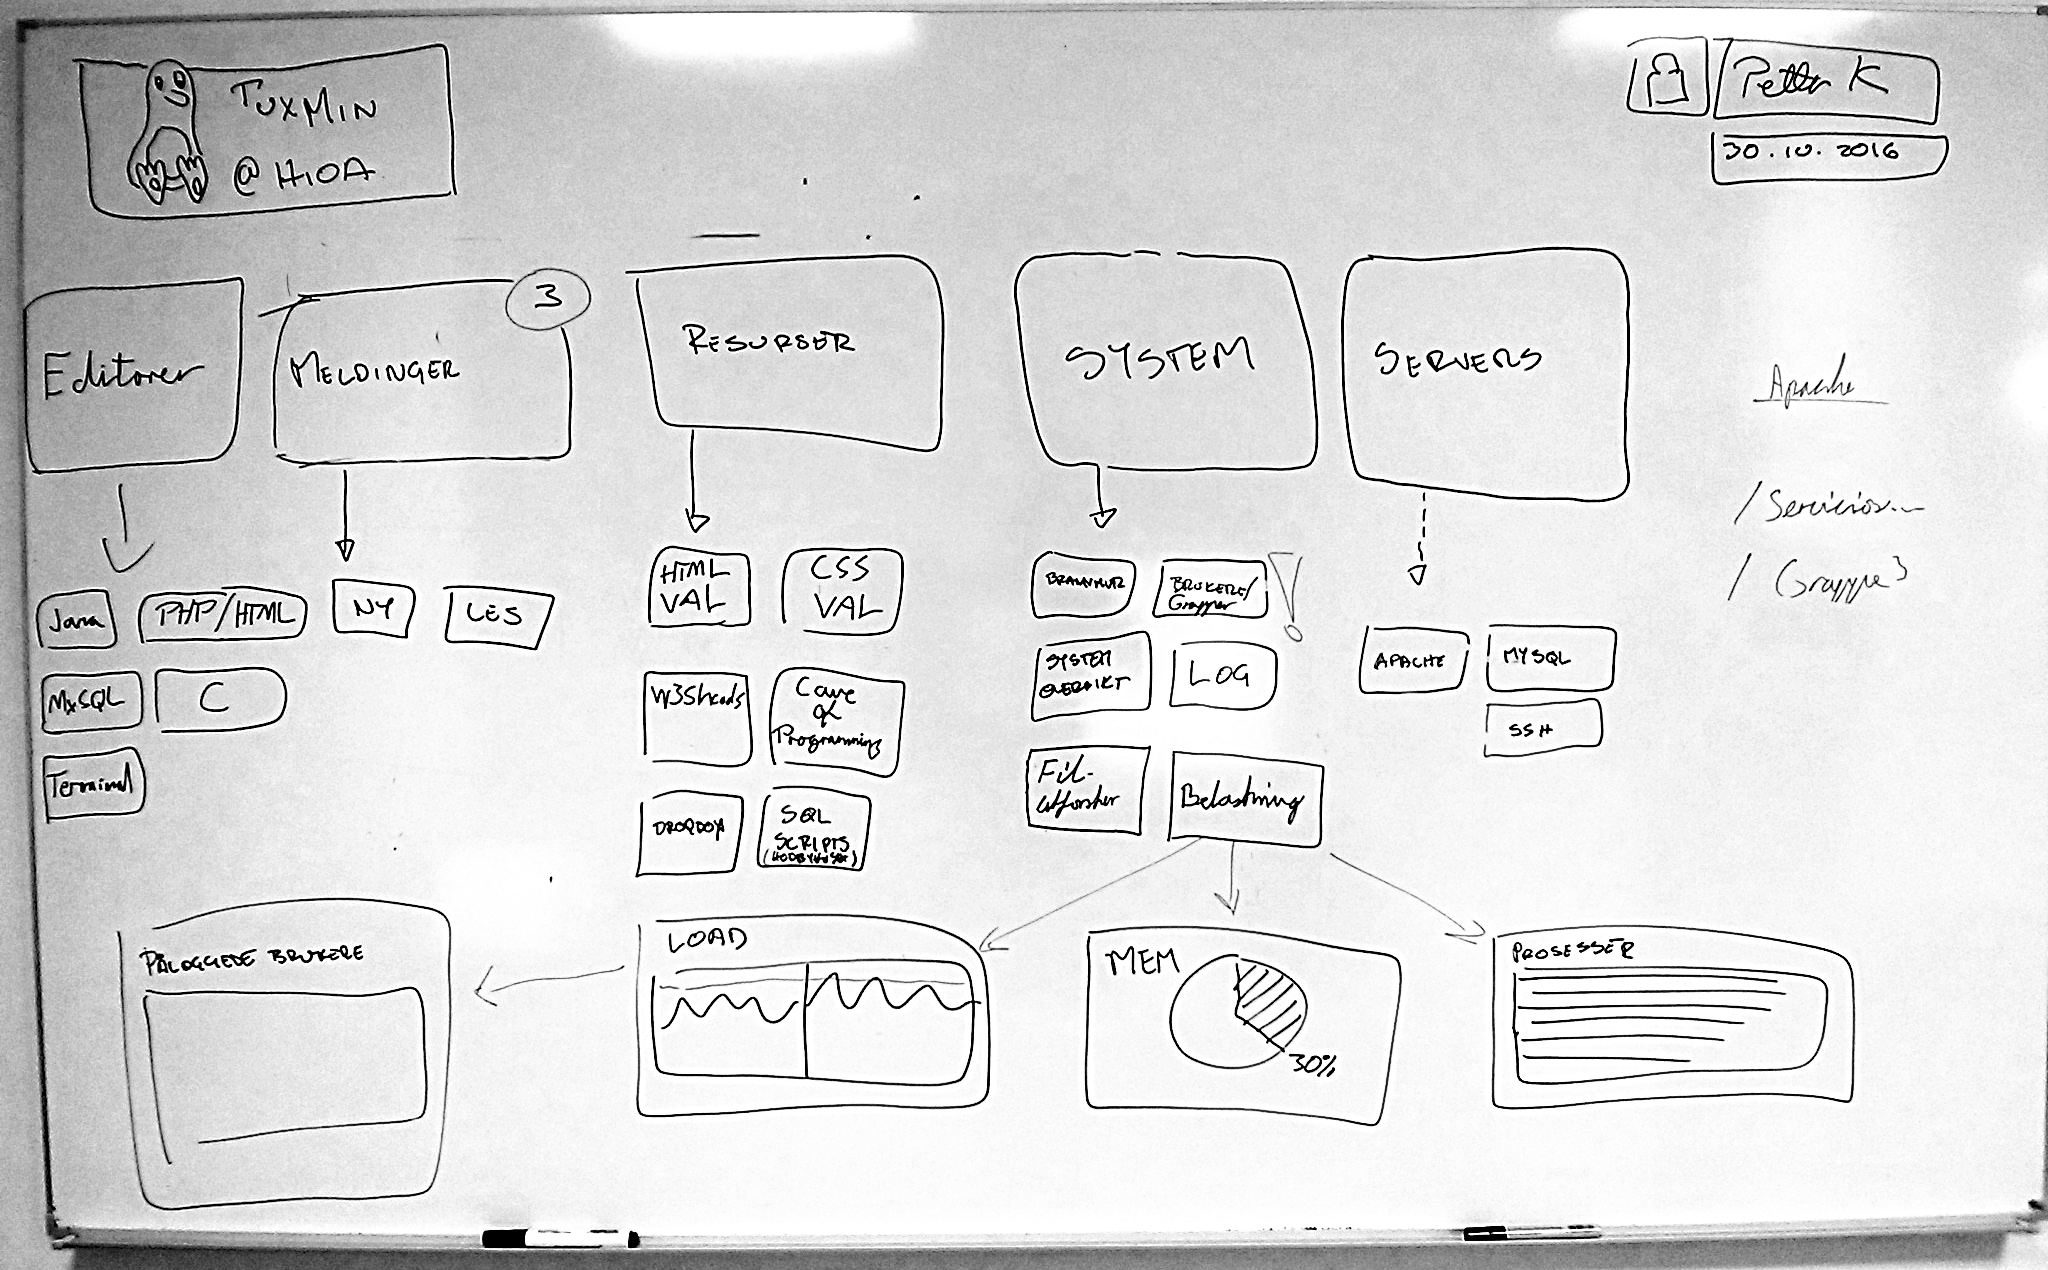
\includegraphics[width=\textwidth,height=\textheight,keepaspectratio]{./img/prosessdokumentasjon/foersteutkast/foerste.jpg}
\caption[Første utkast]{Første utkast over brukergrensesnittet.}
\label{fig:foersteutkast}
\end{figure}

\section{Low-fi prototype}

\section{Hi-fi prototype}

\section{Kriterier og avgjøresler}
Fokuser på alle valg som ble tatt. Hvilke kriterier og 
prinsipper i faget ligger bak avgjørelsene? 

Her kan vi skrive om hvorfor vi har akkuratt valgt Linux. Hvorfor skal løsningen være webbasert og hvorfor skal den kjøres i en virtuell maskin? Og så andre kriterier og avgjøresel som vi har tatt under veien. 
\chapter{Brukertesting}
\lettrine[lines=2]{M}{}ed hensikt å kartlegge samt danne oppfattning om vår tankemåte for produktet og prototypen har vi valgt å gjennomføre brukertester basert på hi-fi prototypen. 
Hensikten med testen er å tydeliggjøre eventuelle fallgroper og mangler som ikke er synliggjort under utvikling av produktet.
Som utvilker har man ikke samme perspektiv eller persepsjon av sin egen produkt som en sluttbruker. Brukertesting vil derfor hjelpe til å forbedre produktets sin kvalitet mot sluttbrukeren.

\section{Gjennomførelse}
Under gjennomførelsen av testet er det ytterst viktig å informere brukeren om at det er ikke brukere som blir testet uten produktet.
Dette er noen alle testpersoner i testen ble informert om. 
Antall testperson som produktet testes på er $5 \pm 2$ individer ettersom frenkvensebilde (fordeling av data) blir normalt densamme også da testpopulasjonen gjøres større.\cite{lazar2010research}\cite{book:utforming}

Testet gjennomførdes slik at brukeren fikk gjennomføre oppgaver basert på de moduler og deler som allerede var implementert i hi-fi prototypen. 
Testet var noe begrenset ettersom få funksjoner var implementert i prototypen under testtilfellet.

Det var forventet at brukertesten vil gi en god henvisning om hvordan de grafiske delene i systemet er utformet.
Brukeren ble presentert med følgende oppgaver:
\begin{description}
\item[Design og navigasjon]
Generell navigasjon i systemet. 
Det ble observert hvordan det er for brukeren å finne frem til de moduler som må aktiveres for å gjennomføre to etterkommende oppgaver i systemet.

\item[Brukeradminstrasjon]
Testpersonen var bedt om å gjennomføre enkel brukeradministrasjon. 
Brukeren fikk spørsmål om de forstod hensikten bak hvert enkelt skjermbilde.

\item[Konfigurasjon av webserver]
Brukeren fikk teste modulen for konfigurasjon av \textit{Apache} webserver. 
Testet ble gjennomført med brukere som ikke hadde større eller noen erfaring med slike oppgaver.
Det bli undersøkt dersom brukeren forstår hvert skjermbilde og kan forklare hva som er hensikten med alle trinn.
\end{description}

Testpersonen fikk tre oppgaver basert på alle de over nevnte testområder for systemet.
De praktiske oppgavene ble utformet på følgende måte:
\begin{enumerate}
\setlength{\itemsep}{1pt}
\setlength{\parskip}{0pt}
\setlength{\parsep}{0pt}

\item Bruk én stund på å gjøre deg kjent med grensesnittet. Når du synes at du blitt kjent med konfigurasjonen kan gå videre til neste oppgave.
\item Forsøk å konfigurere brukergrupper. Du skal legge til en ny brukergruppe og tildele noen resurser til den gruppen.
\item Din siste oppgave blir å konfigurere \textit{Apache} webserver. 
Du skal legge til en mappe som skal være tilgjengelig for serveren. 
Etterpå skal du aktivere funksjonen <<directory browsing>> for de mapper du har valgt og aktivere en \textit{PHP} modul for webserveren.
\end{enumerate}

Testene gjennomføres etter prinsippet <<\textit{think out loud}>> som medfører i enkle trekk at testepersonen forteller hva de tenker gjøre i hver situasjon når oppgavene gjennomføres. 
Dette var en nødvendig tilnærming ettersom dialogboksene i systemet hadde ikke fungerende komponenter (f.eks. knapper, lister eller sjekkbokser).

Testpersonen ble derfor presentert med kun en representasjon av et påtenkt fremtidig grensesnitt. 
Alle trinn som brukeren gjennomfører ble notert notert. 
Under forsøkene fik testpersonen ingen hjelp med gjennomføring av oppgavene.

\section{Spørsmål}
Testpersonen ble presentert med et flertall spørsmål som var plassert under hver tilhørende kategori. 
Følgende er en liste på de spørsmålene ble valgt for brukertesting.
\begin{enumerate}
\setlength{\itemsep}{1pt}
\setlength{\parskip}{0pt}
\setlength{\parsep}{0pt}
\item Navigasjon
\begin{enumerate}
\item Følte du at det var intuitivt å navigere deg i systemet?
\item Var det vanskelig å finne frem til deler etterspurt i oppgaven?
\end{enumerate}
\item Design og Layout
\begin{enumerate}
\item Hvordan opplevdes layouten?
\item Hvordan opplevde du bruk av farger?
\item Er det noen logikk i hvordan alle elementer er plasert på siden?
\item Er grafiske elementer som undermenyer logisk integrert i hverandre?
\end{enumerate}
\item Brukeradministrasjon
\begin{enumerate}
\item Har du noen erfaring med brukerkonfigurasjon på datamaskiner eller andre system?
\item Hvordan opplevede du prosessen for brukeradministrasjon?
\item Var noen av de trinnene vanskelig å forstå?
\end{enumerate}
\item Konfigurasjon av webserver
\begin{enumerate}
\item Har du noen erfaring med konfigurasjon av webservere?
\item Hvordan opplevde du prossessen over konfigurering av webserver?
\item Var noen av de trinnene vanskelig å forstå?
\end{enumerate}
\item Generelt
\begin{enumerate}
\item Hva jobber du med?
\item Hvor lang generell erfaring har du med å bruke datamaskiner?
\item Bruker du mest datamskin eller en tablet?
\item Har du noen erfaring fra systemadministrasjon?
\item Har du noen erfaring med programmering eller utvikling?
\end{enumerate}
\end{enumerate}

\section{Testresultat}
Testene ble gjennomført på hi-fi prototype plasert på en publikk webserver under adresse:\\ \url{http://student.cs.hioa.no/~s198569/EasyDev/login.php}\\
\textit{Det er ikke nødvendig med brukernavn eller passord for pålogging}.

Det ble totalt testet 7 personer på plass i kaféen ved Pilestredet 35. 
Den testede gruppen bestod av kun studenter fra linjer som data, bygg og økonomi.

\subsection{Hva er bra?}
Alle brukere gjorde seg rask kjent med måten systemet skal brukes på.
Samtlige testpersoner mente at det var ganske enkelt å navigere seg på startsiden uten å behøve <<tenke>>. 
Det vat ment at layouten føltes intuitivt på en måte der de fleste kjenner seg igjen fra bruk av andre systemer (f.eks. generelt plassering av ikoner på et nettbrett). 
Ingen av testpersonen testperson hadde problem med å finne nødvendig modul i grensesnittet for å gjennomføre gitt oppgave.
De fleste testpersoner mente at layouten og brukervennligheten var meget god.

Alle testpersoner klarte å sette opp alle funksjoner som ettersportes for oppsett av webbserver. 
Dette var uavhengig hvis de var kjent med de spesifikke underliggende modulene. 
Brukerne ble bedt om å aktivere en spesifikk modul utefra dess funksjon.
Dette var noe som alle brukere klarte ettersom navnet på modulene gav en henvisning til modulens spesifikke funksjon (f.eks. modulen \textit{Ruby} aktiverer faktisk ruby funksjonalitet på serveren osv.).

Det var kun positive tilbakemeldinger i forhold til bruk av farger. 
Største delen av testpersoner mente at de brukte fargene gav en behagelig inntrykk som bidrar til en forhøyd brukeropplevelse.

\subsection{Hva bør forbedres?}
Noen brukere mente at layouten borde gjøres mer visuelt tiltalende ettersom foreløpig gav den inntrykk over et uferdig produkt.
Det var noen mindre problemer med å konfigurere grupper, det var enkelte testpersoner som ikke skjønte helt hensikten med brukergrupper i systemet. 
Densamme gjelder da det skulle tildeles resurser til en gruppe. Det kan eventuelt skylles at vi har plassert flere valg som kan gjøres direkte fra modulen for gruppeadministrasjon (se fingur \ref{fig:brukerehi2} side \pageref{fig:brukerehi2}).

Flertall brukere hadde også utfordring med å forstå hvordan man bruker neste trinn i gruppeadministrasjon (bilde \ref{fig:brukerehi3} side \pageref{fig:brukerehi3}). 
For noen var det uklart dersom hensikten var å kun legge til brukere eller hvis man kunde også legge til grupper i én og samme skjermbilde.
Årsaken til dette er at bildet har en forhåndsdefinert liste som består av både brukernavn og programmoduler. Noe som gav litt uklart inntrykk relatert til bruksområde.

I bilde \ref{fig:brukerehi4} (side \pageref{fig:brukerehi4}) var det noen uklarheter angående til hvilken gruppe som man egentlig legger til modulene. Dette framgår i titteln for vinuduet men noen av testpersonen mente at det borde gjøres mer tydelig. 

Generelt i administrasjon av grupper var det noe forvirrende med at vi hadde lagt til to <<\textit{tilbake}>> knapper på begge sider av dialogvindu. Det viste seg være noe så uklart gjeldende hvilken hensikt disse to knapper har. Fra et brukerperspektiv ser det ut som at begge knapper leder til et og samme trinn i dialogen. 
Dette er helt riktig da den venstre knappen leder <<\textit{tilbake}>> og høyre <<\textit{frem}>> leder til neste trinn i dialogen og selve \textit{label} er feil på en av knappene. Feilet skal utbedres under neste revisjon.

Dialogvinduene er utformet slik at det skal ikke være mulig å gjøre noen feil eller at dialogen skal avsluttes midt i prosessen, det vil si for tidlig.
Foreløpig er dialogene satt opp slik at hvis bruker klikker utenfor dialogvinduet kommer forårsake lukking av det vinduet. 
Det var noe som inntruffet flere ganger under brukertesten. 
Noen av testpersonen opplevede det som frustrerende. Hvis man f.eks. jobbet med vindu nr. 3 av 4 i dialogprosessen måtte hele prosessen påbegynnes på ny dersom vinduet ble plutselig lukket på grunn av et feilklikk. 

Det ble mottatt flere tilbakemeldinger gjeldende den generelle måten å vise dialoger til brukeren. Testpersonene mente når en dialog vises bør den være dominerende over de elementer som ligger i bagrunn.  
De bakliggende komponentene borde derfor tones ned, slik at disse ikke lengre er <<forstyrrende>> for den oppgave som skal gjennomføre.
Det er derfor tenkt at det skal implementeres et underliggende lag som er halv-gjennomsiktig og ligger bak dialogboksen slik at andre komponenter som ikke er i bruk blir plassert i andre plan.
\chapter{Evaluering}
\lettrine[lines=2]{P}{} roduktet vi sitter igjen med etter alt arbeidet er utført er noe annerledes enn det vi så for oss da vi begynte å jobbe med prosjektet. Ambisjonene våre var rettet mot å lage et så godt produkt som mulig, samt å implementere noe funksjonalitet i dybden for å gi brukeren en følelse på hvordan sluttproduktet kunne se ut og hvordan det ville være å jobbe med det. Dette kapittelet vil berøre alle aspektene ved produktet, hvorfor det ble som det ble og hva vil ville ha gjort annerledes.

\section{Produktet}
Resultatet av HiFi-prototypen er det som vi anser som produktet vårt. Den er dog en dårlig pekepinn på hva prosjektet går ut på og dermed vil denne rapporten være det viktigste bidraget til sluttproduktet vårt. Uten rapporten og historien som følger med rundt beslutningene som ble gjort og prosessen underveis vil ikke prototypen ha noen verdi. Prototypen må derfor sees i lys av det man leser i rapporten.


\section{Begrensninger}
Dette punktet har vært den største utfordringen vi har støtt på. I et prosjekt der man skal lage noe ønsker man å har et produkt man kan være fornøyd med, og som vi kunne tenke å jobbe med selv. Dette var jo målet vi hadde satt oss også, men det ble klart ganske tidlig at vi måtte omprioritere, lage ny fremdriftsplan og sette nye mål på hva vi kunne få til innenfor angitt tid.
Den største utfordringen det medførte var i hvor stor grad vi skulle implementere funksjonalitet. Om vi hadde hatt tid kunne vi implementert veldig mye av funksjonaliteten, i alle fall i brukergrensesnittet, men det har altså ikke vært mulig innenfor tidsrammene.
Resultatet har da blitt at vi videreutvikler mockup/prototype fra første innlevering og viser prototypen i "ny drakt" slik at man får en bedre, mer funksjonell prototype, men som ikke har mer funksjonalitet implementert.\\
Vi har prøvd å forholde oss til prinsipper for MMI-faget. Først og fremst har vi jobbet med farger som passer godt sammen, samt laget en oversiktlig meny som gir brukeren rask tilgang til de forskjellige kategoriene av funksjonalitet vi har ønsket å implementere.
Da produktet vårt er av en teknisk art og ikke ment for den jevne bruker vil ikke alle menypunkter være selvforklarende, men at man har en liten "læringskurve" for å bli vant med produktet slik at man kan utnytte all den funksjonalitet produktet tilbyr.
Det skal likevel ikke være behov for å kunne alle disse avanserte funksjonene for at man kunne bruke systemet på en tilfredsstillende måte.


\section{Hva ville vi ha gjort annerledes?}
Premisset for prosjektoppgaven i MMI er annerledes enn det vi la opp til da vi kom opp med vår idé, som var før oppgaven hadde blitt delt ut. Dette har medført at vi ikke fikk tid til å utvikle løsningen vår slik vi ønsket i utgangspunktet, men i vi stedet tilpasset produktet vårt til oppgavens spørsmål og krav.
Det medførte til at vi laget et forslag mer som en konseptløsning med god dokumentasjon som viser ideene og ambisjonene våre i stedet for å lage et best mulig sluttprodukt med mest mulig funksjonalitet. Vi ville likevel stå i fare for å ikke ha tid til å gjøre ferdig produktet eller komme med en god nok løsning som rettferdiggjorde valgene vi hadde tatt.\\
Videre kunne vi tenkt oss å tatt med en brukerundersøkelse før vi begynte arbeidet for å se hva andre studenter kunne se for seg for løsninger og funksjonalitet. Det ville ikke påvirket arbeidet vårt i nevneverdig grad, men det ville vært interessant å ta med flere av de resultatene inn som tiltenkt funksjonalitet i produktet.


%Appendix for vedlegg og andre ting som ikke direkte passer inn i resten av rapporten

\bibliographystyle{plain}
\bibliography{bibliografi}
\addcontentsline{toc}{chapter}{Vedlegg}
\appendix
\chapter{Funksjonalitet} \label{app:funksjonalitet}
Følgende tillegg beskriver i detalj noen av modulene som er tenkt at systemet skal inneholde ved første release.


\section{Tjenere (servers)}
Følgende modul skal brukes til å sette opp forskjellige servere på maskinene. Modulene kjøres som skript og setter ønsket funksjonalitet etter ønske. Under oppsettet av hver enkel tjener blir brukeren presentert med en “wizard” der man får lov til å velge ekstra funksjonalitet eller annen funksjon som eventuelt tilbys av programvaren (f.eks. virtuelle servere i Apache). Oppsett av tjenere er fullstendig modulbasert. Dette medfører at brukere kan etter ønske utvikle egne konfigurasjonsmoduler som kan publiseres og deles med andre studenter via systemets marketplace. 

\subsection{Apache webserver}
Modulen setter opp og konfigurerer apache webserver med tilhørende moduler. Brukeren blir presentert med en wizard som går igjennom følgende innstillinger og konfigurasjoner.
\begin{description}

\item[Mapper] Her kan brukeren sette opp hvilke mapper som skal være tilgjengelige på nett. Brukeren har mulighet til å sette opp flere mapper i sin hjemmemappe samt se en forhåndsvisning på hvordan nettadressen kommer til å se ut. Dersom brukeren har satt opp synkroniseringstjeneste (mer om dette under ...) blir det også mulig for brukeren å “peke” webserveradresse til en mappe i synkroniseringstjenesten. Dette vil da gjøre det mulig for brukeren til å oppdatere nettsiden fra en ekstern datamaskin som synkroniserer til samme tjeneste.

\item[Tilgang og sikkerhet] Her er det mulig å sette opp funksjoner som “directory browsing” og diverse sikkerhets innstillinger.

\item[Moduler] Aktivering av tilleggsmoduler som php og MySQL støtte. Valg av feks disse to vil laste ned og installere php samt MySQL database med standardinnstillinger.
\end{description}

\subsection{MySQL}
Modulen installerer, og setter opp bruker med samme brukernavn og passord som systemets  bruker. Etter ønske blir det også vist en “wizard” som viser brukeren hvordan man kan koble opp mot databasen og bruke denne. Etter ønske fra brukeren kan det også bli satt opp med software for enklere administrasjon av databasen, f.esk. MySQL Workbench. Det skal også gis mulighet til å konfigurere tabeller som brukes i fag som Databaser (se her etterkommende avsnitt om hobbyhuset). 

\subsection{SSH}
Alle *NIX baserte system kan kontrolleres via “secure shell”. Denne modulen vil sette opp en standard ssh-server på maskinen som gjør det mulig for brukeren å logge seg på fra en ssh klient.

\section{System}
Modulen system innholder moduler som brukes til systemkonfigurasjon og kontroll. Modulene her kan brukes til installere og konfigurere både programvare og medfølgende innstillinger på brukerens sin virtuelle maskin. 

\subsection{Programvare}
Her kan brukeren velge å installere moduler som er tilgjengelige via et sentralt repository for EasyDev. Brukeren kan velge å laste ned og installere nye moduler (programvare) eller slette en eksisterende modul.

\subsection{Oppstart}
Modulen gir brukeren mulighet til å velge hvilke prosesser som skal startes sammen med systemet. For eksempel dersom man ønsker at sammen med systemet skal startes Apache webserver og MySQL database. Dette velges utfra en liste med sjekkbokser som generes basert på de moduler som er installert på systemet.

\subsection{Brannmur}
Dersom man ønsker at systemet skal ha en brannmur blir det mulig for brukeren å sette opp slik funksjonalitet via brannmurmodulen. Brukeren kan med hjelp av denne modul implementere en brannmur som må ta høyde for de moduler som allerede kjører på systemet. Dette må gjøres for at brannuren ikke skal sperre eventuelle porter for inngående kommunikasjon som de ulike modulene bruker. Derfor skal det finnes en intern fil (eller database) som innholder all nødvendig informasjon om porter som skal holdes åpne dersom brannmuren blir konfigurert i etterkant. Oppsett av brannmuren skal foregå med hjelp av en “wizard” og konfigurasjons-gui der brukeren kan kontrollere de innstillinger som blir foreslått basert hvilken port som skal holdes åpen. Alle kommandoer som kjøres fra GUI skal også presenteres for brukeren i en nærliggende utskriftsvindu og i tillegg lagres i en loggfil. Hensikten med dette er at man skal ha mulighet til å studere den “manuelle” konfigurasjonen for egen læring.

\subsection{Brukere og grupper}
Her definerer man brukere og grupper og hvilke brukere som er med i hvilke grupper.
Denne modulen er tenkt brukt sammen med “Ressursene”, det vil si webområdene man har definert og databasene man har opprettet osv. 
Man kan her opprette brukere og legge dem i grupper. Gruppene kan da brukes som prosjektgrupper, og man får opp en liste med ressurser på maskinen der man kan huke av hvilke ressurser gruppen skal ha tilgang til. De brukerne som er medlemmer i gruppen vil da få redigeringsmulighet på de delte ressursene og mulighet til å laste opp og endre innhold.
Dette er en sentral funksjonalitet i forhold til å gi studentene en god plattform å jobbe med i prosjektoppgaver, og så langt vi har oversikt over er det en unik funksjonalitet som ikke tilbys i andre løsninger, hverken på HIOA eller i administrasjonsløsninger for Linux.

\subsection{Synkronisering}
Modulen skal gi mulighet for brukeren til å sette opp synkronisering til de mest vanlige skytjenestene som Dropbox, SkyDrive, Google Drive men også eventuelt hjelpe til å sette opp MyCloud dersom noen ønsker å benytte seg av en egen synkroniseringsløsning. 
Det skal være mulig å dele mapper innad i en gruppe. Tanken er at brukere kan direkte skrive inn gruppemedlemmenes studentnummer for å sende forespørsel til en synkronisert mappe. Denne funksjonen er mest sannsynlig kun mulig dersom man kjører en synkroniseringssky internt på skolens sine servere. 

\subsection{Systemoversikt}
Her skal det bli presentert forskjellige typer av systeminformasjon, som informasjon om aktuell OS kjerne, antall brukere, installerte moduler og tilgjengelig lagringsplass på samtlige partisjoner. 

\subsection{Logg}
En modul som tydelig viser all loggføring som foregår i “/var/log”. Det skal være enkelt for brukeren å identifisere hvilket program loggen kommer fra. Et eksempel er loggen fra Apache som er plassert i “/var/log/httpd.log”. Dette er selvsagt ingen brukervennlig måte å identifisere en loggfil. Brukeren skal ha mulighet til å velge at man ønsker å se loggfilen for Apache server, og man får så opp filens innhold og hvor filen er lagret på systemet. Det skal også være mulig å lese gamle loggfiler som har blitt komprimert av loggrotasjonsystemet. Det vil også være mulighet for å søke i loggfilene.

\subsection{Belastning}
Skal være en form av “widgets” og/eller statistikk som presenteres for brukeren om systemets “helse” og tilstand. Her skal det være mulig å lese av CPU belastnintg, tilgjengelig hukommelse, aktuelle operasjoner på platelager og prosessenes belastning. Man skal også få opp nettverksinformasjon og belastningen på de forskjellige enhetene.



\section{Ressurser}
Modulen består av forskjellige ressurser som kan være til god nytte i forskjellige fag. Det kan være alt fra gode linker til nettsider, til forskjellige verktøy som validering av kode. Innholdet her blir mest sannsynlig manuelt lagt til av studentene, avhengig av hvilket fag som er interessant for dem. Målet er også at modulene eventuelt kan utvikles av studentene selv slik at disse blir godt tilpasset til de fag som gis ved skolen. Det skal være mulig å rangere alle modulene etter for eksempel antall stemmer eller popularitet (antall nedlastninger).

\subsection{Validering}
I de fleste fag som har med webutvikling å gjøre er det krav at man skal validere oppgavene  man har laget slik at løsningen følger alle nødvendige standarder. Det er tenkt at under ressurskategorien skal det finnes tilgjengelig en modul som tillater å velge godkjente filtyper og kjøre online validering på disse. Dette vil da gjøre det enklere å raskt validere filene uten å  gjøre dem tilgjengelig/publisere på en webbserver eller laste dem opp til en tredjeparts side for validering.

\subsection{Nettressurser}
Mulighet for en rask tilgang til gode kunskaps resurser på nettett sortert etter fag. Dette kan for ekesempel være W3Shools, Udemy, Cave of Programming med mer.

\subsection{Regex-generator}
Det finner mange regex-generatorer tilgjengelige på nettet. Problemet med disse er at selve syntaksen for hvordan regexen skal valideres på de forskjellige sidene varierer. Med andre ord det tar tid å lære seg den enktlte regex validator som finnes på nettet, og som ofte krever disse at brukeren kan noe standard regex syntaks fra før. Det som skal tilbys via vårt system er at brukeren skal få mulighet til å bygge sin egen regex ut fra et enkelt grafisk grensesnitt som er en form av “logiske gater” eller “Venn” diagram der man skal angi hvilke typer av ASCII eller uttrykk som skal inkluderes eller ekskluderes for den aktuelle regex-streng. Ut over dette skal det også være mulig for brukeren å skrive inn sin egen regex og direkte teste denne den på ønskede strenger for å se om den fungerer. Eventuelt kan det implementeres en link til ressurser som viser hvordan regex kan implementeres i forskjellige språk og teknologier. Alt fra tolkningsrpåk som PHP, JavaScript til kompileringsspråk og de mest vanlige grafiske bibliotek som Swing, JavaFX, GTK+ eller Qt.

\subsection{SQL scripts}
Her kan det plasseres SQL-script som for eksempel “hobbyhuset” som kan brukes i faget Databaser. Andre script som backup av databaser, samt andre administrative script vil også finnes her.

\subsection{Versjonshåndtering}
Det er normalt ganske vanskelig å komme igang med et versjonskontrollsystem. En modul som ikke bare setter opp en av de mest populære versjonhånderingssystemene (f.eks. GIT) men også viser de mest vanlige prinsippene som er nødvendig for å starte med å jobbe i team der man bruker versjonshåndtering. Det kan være elementer som oppsett, staging, commits, branching, merging, diff samt push og pull til fjernservere. 



\section{Meldinger}
En integrasjon av studentepost direkte til systemet. Det skal tilsvare mer eller mindre samme funksjonalitet som i en webmail. 



\section{Verktøy}
Modulen skal bestå av praktiske verktøy som kan være til god hjelp dersom man trenger å gjøre endringer i konfigurasjon direkte på den virtuelle maskinen. Foreløpig tenker vi på de to verktøy som er til grunn og bunn viktigst for alle brukere: teksteditor og terminal.

\subsection{Editorer}
Integrert teksteditor som kan brukes til de fleste utviklingsspråk, med syntakshighlighting og syntakskontroll. En slik editor mest aktuell for språk som brukes i webutvikling ettersom det blir mulig å utvikle direkte på webserveren uten å koble til/montere mappen eller laste opp filene kontinuerlig til serveren. Editoren skal også gi mulighet til å kompilere kode. Dersom man bruker skriptspråk som html eller css skal det være mulig å validere syntaksen direkte fra editoren. Eventuelt skal det også implementeres støtte for versjonshåndtering. Eksempel på språk og script som skal støttes: Java, JavaScript, PHP, Html, SQL, CSS, C, bash.

\subsection{Terminal}
For å gjøre det enkelt å administrere systemet for mer erfarne brukere skal det også tilbys en modul som representerer en terminalemulator. Foreløpig er det noe uklart hvordan en slik terminal skal implementeres i en nettleser ettersom det er ønskelig å gir umiddelbar tilbakemelding til bruker som utskrift av resultat fra de kommandoer som kjøres i terminalen. Målet er å gi like god bruksopplevelse som man får ved bruk av terminal direkte på maskinen. 

\subsection{Filbehandler}
En enklere variant av en filbehandler som tillater bruker til å behandle filer på systemet sitt. Programmet skal følge samme rettigheter som man har på systemet slik at vanlige brukerrettigheter får brukeren kun behandle filer i sin egen hjemmemappe. Dersom man ønsker “root”-tilgang må man logge seg på med “root”-passord, dette vil gi en tilbakemelding til brukeren i form av at f.esk. programmet skifter farge til rød (skal signalisere fare ettersom med “root” tilgang er det fullt mulig å ødelegge systemet). 


Med tanke på læring er det viktig at brukeren kan se terminalutskrift for alle kommandoer som blir foretatt for filbehandlingsoperasjoner. Med andre ord, programmet skal oversette det som brukeren ønsker å gjøre grafisk i programmet til “bash” kommandoer. Eksempel på dette er hvis man ønsker å skifte navn på filA.txt til filB.txt vil brukeren bli presentert samtidig som operasjonen utføres med en utskrift ved siden som viser selve syntaksen for operasjonen. I dette tilfellet : \texttt{bash\$ mv filA.txt filB.txt}. Dette vil gi veldig god forståelse og eksempler på bruk av terminal i unix/linux/mac-miljøer.
\addcontentsline{lof}{chapter}{Tillegsfigurer}
\chapter{Prototyper}
I dette avsnitt blir det nærmere presentert bilder av prototyper. Hensikten er at vi ønsker å presenter bildene i bedre kvalitet enn hva som tillates inne i rapporten. Derfor valgte vi å plassere disse i spesill appendiks.
\section{Low-fi prototype}

\section{Hi-fi prototype}
\begin{figure}[ht]
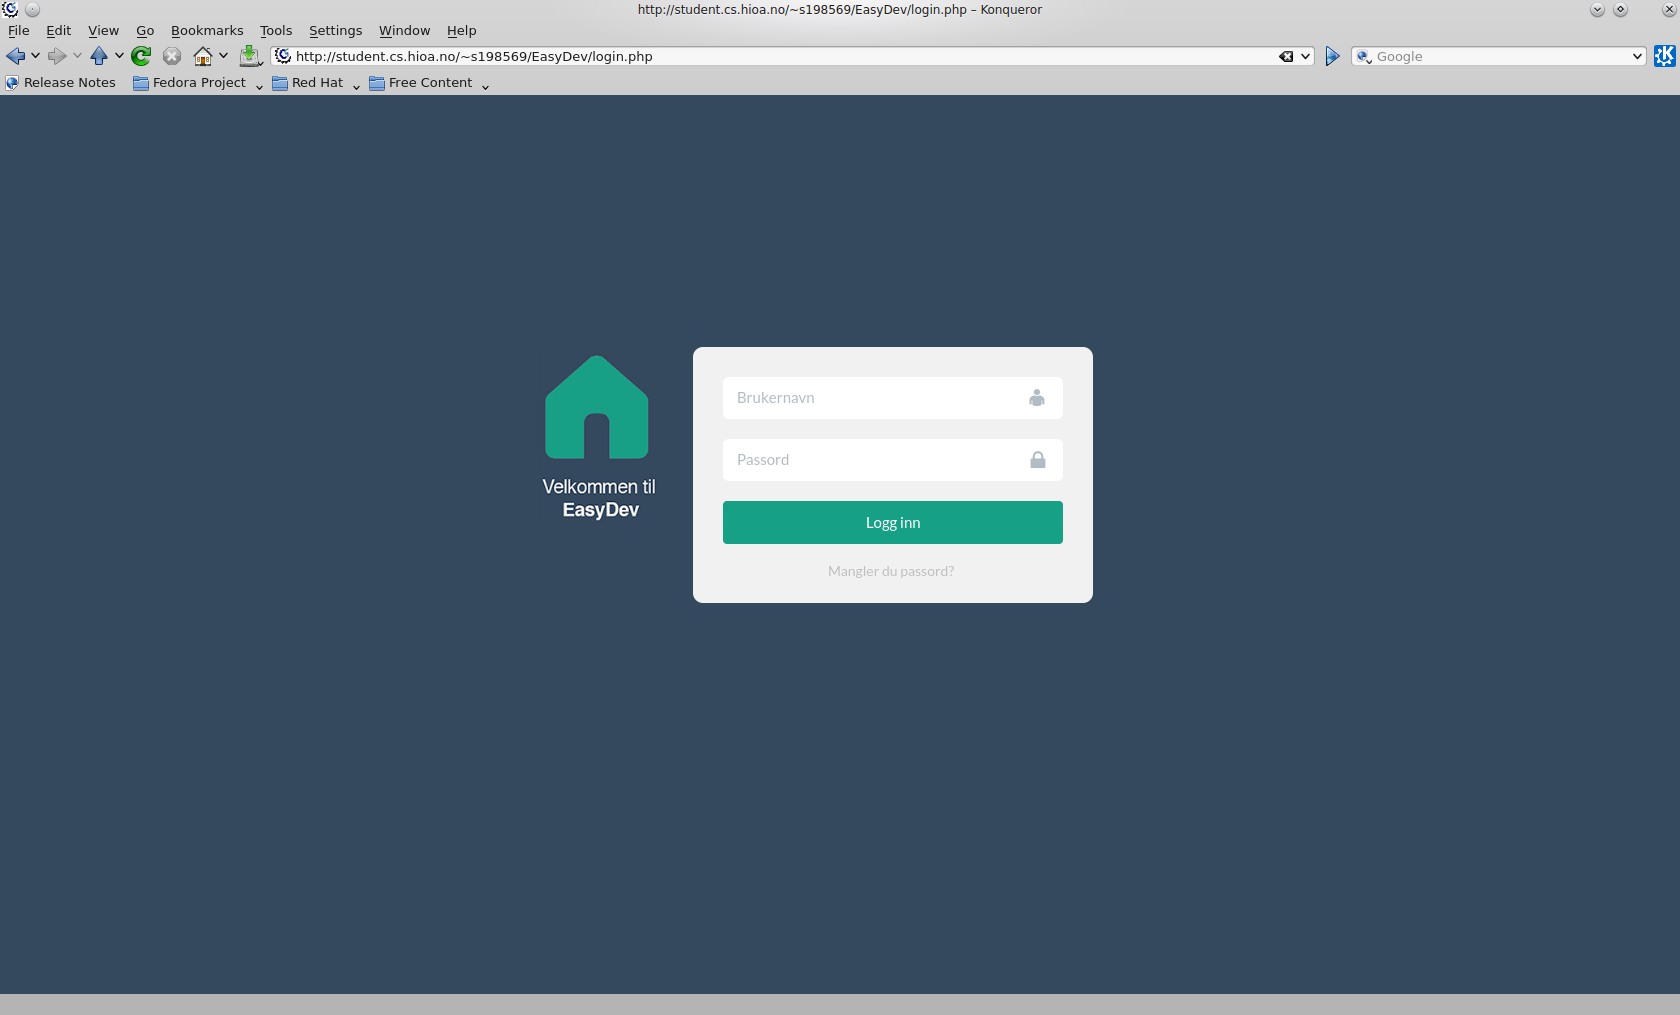
\includegraphics[width=\textwidth,height=\textheight,keepaspectratio]{./img/prosessdokumentasjon/hifi/login.png}
\caption[(Hi-fi) Påloggingsbilde]{Påloggingsbilde. I prtotypen er det mulig å logge seg på uten brukernavn eller passord. Etter dette påloggingsbilde blir brukeren forflyttet til fremside.}
\label{fig:loginhi}
\end{figure}

%KONFIGURASJON AV APACHE
\begin{figure}[ht]
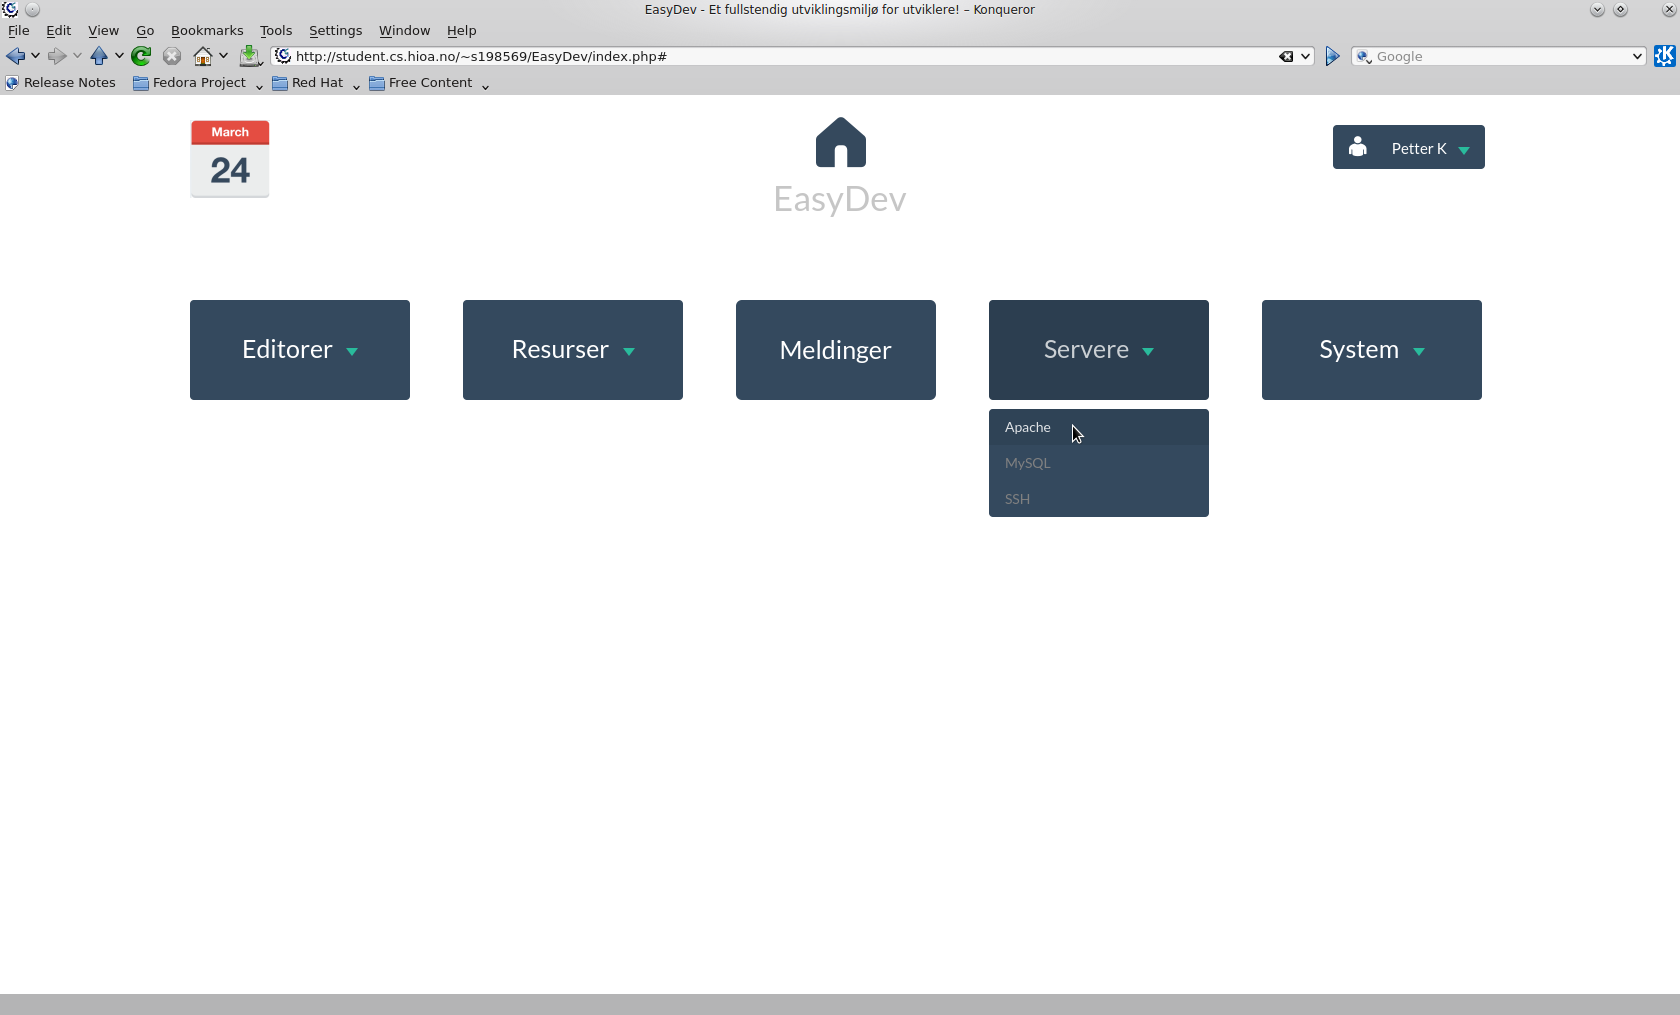
\includegraphics[width=\textwidth,height=\textheight,keepaspectratio]{./img/prosessdokumentasjon/hifi/a1.png}
\caption{(Hi-fi) Webserver: }
\label{fig:apachehi1}
\end{figure}

\begin{figure}[ht]
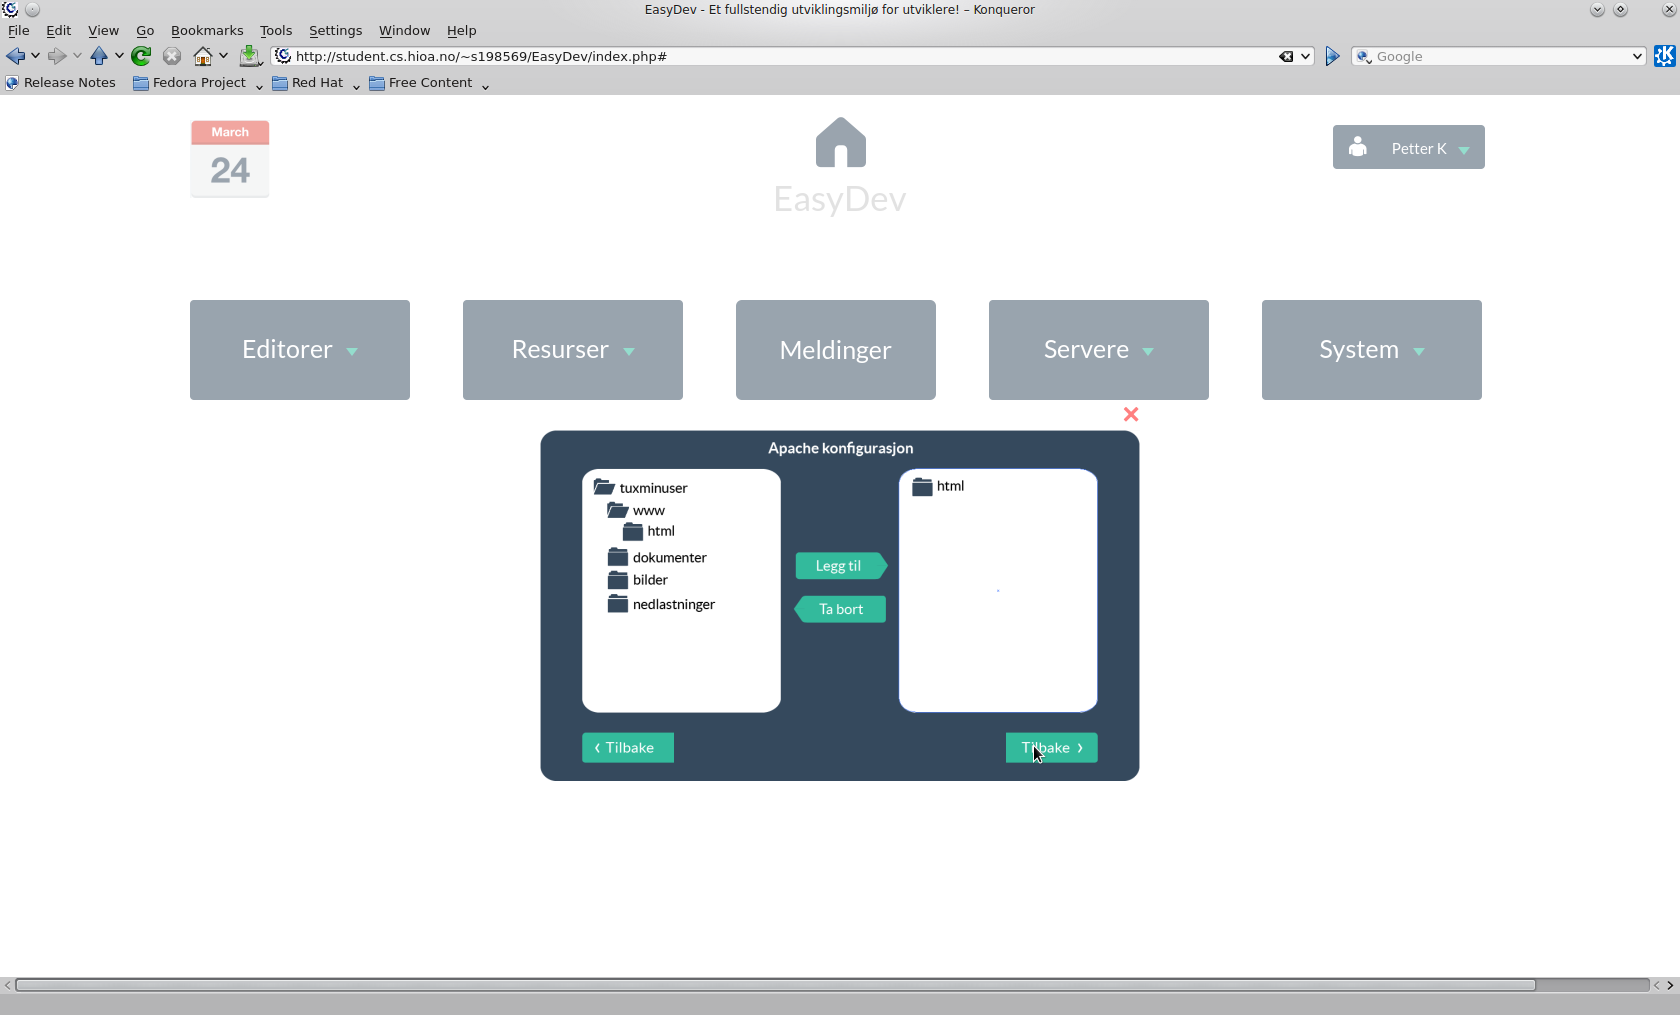
\includegraphics[width=\textwidth,height=\textheight,keepaspectratio]{./img/prosessdokumentasjon/hifi/a2.png}
\caption{(Hi-fi) Webserver: }
\label{fig:apachehi2}
\end{figure}

\begin{figure}[ht]
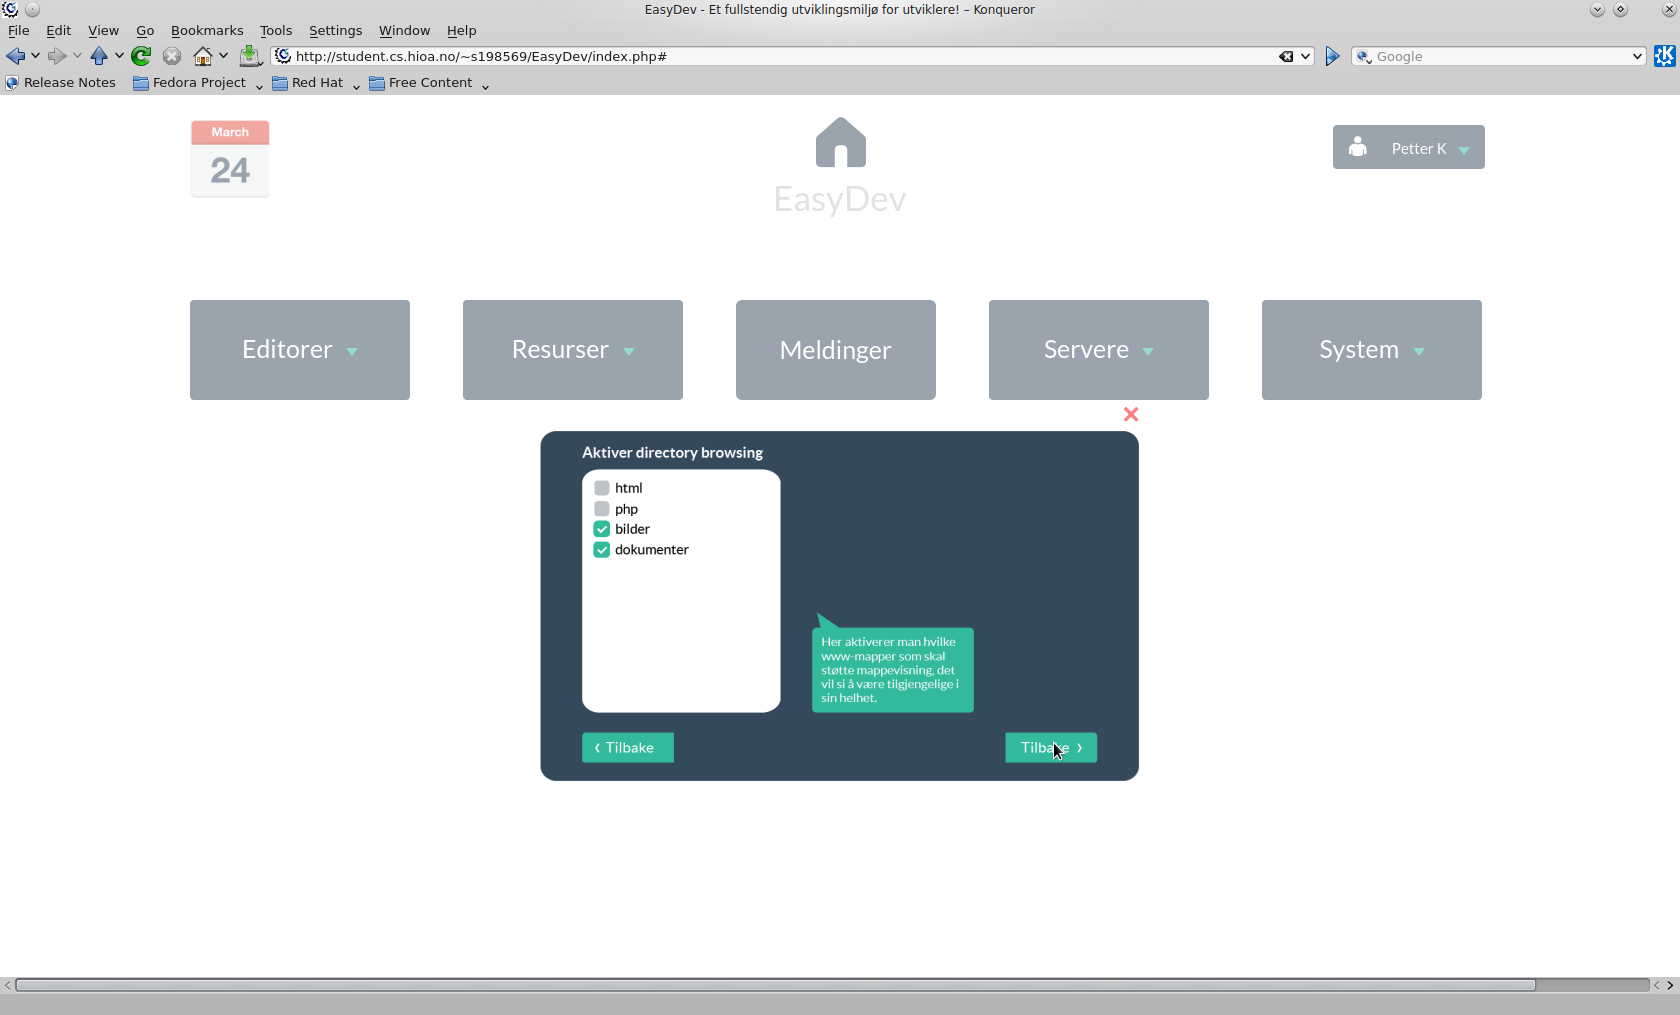
\includegraphics[width=\textwidth,height=\textheight,keepaspectratio]{./img/prosessdokumentasjon/hifi/a3.png}
\caption{(Hi-fi) Webserver: }
\label{fig:apachehi3}
\end{figure}

\begin{figure}[ht]
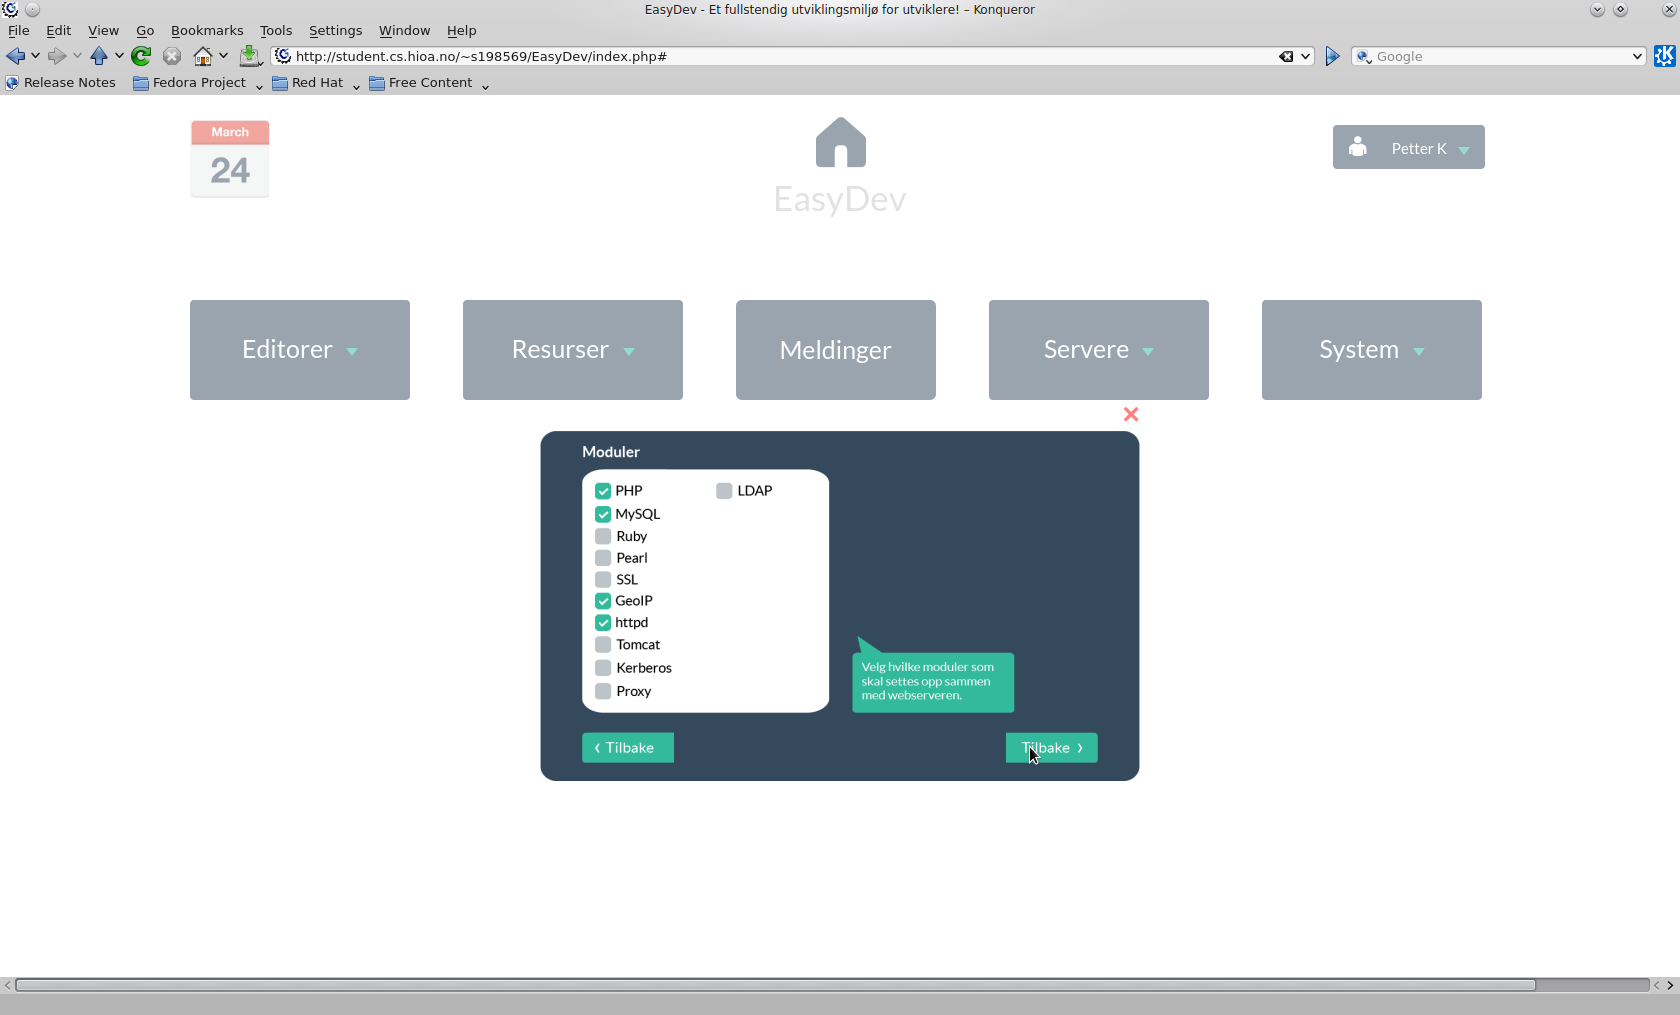
\includegraphics[width=\textwidth,height=\textheight,keepaspectratio]{./img/prosessdokumentasjon/hifi/a4.png}
\caption{(Hi-fi) Webserver: }
\label{fig:apachehi4}
\end{figure}

\begin{figure}[ht]
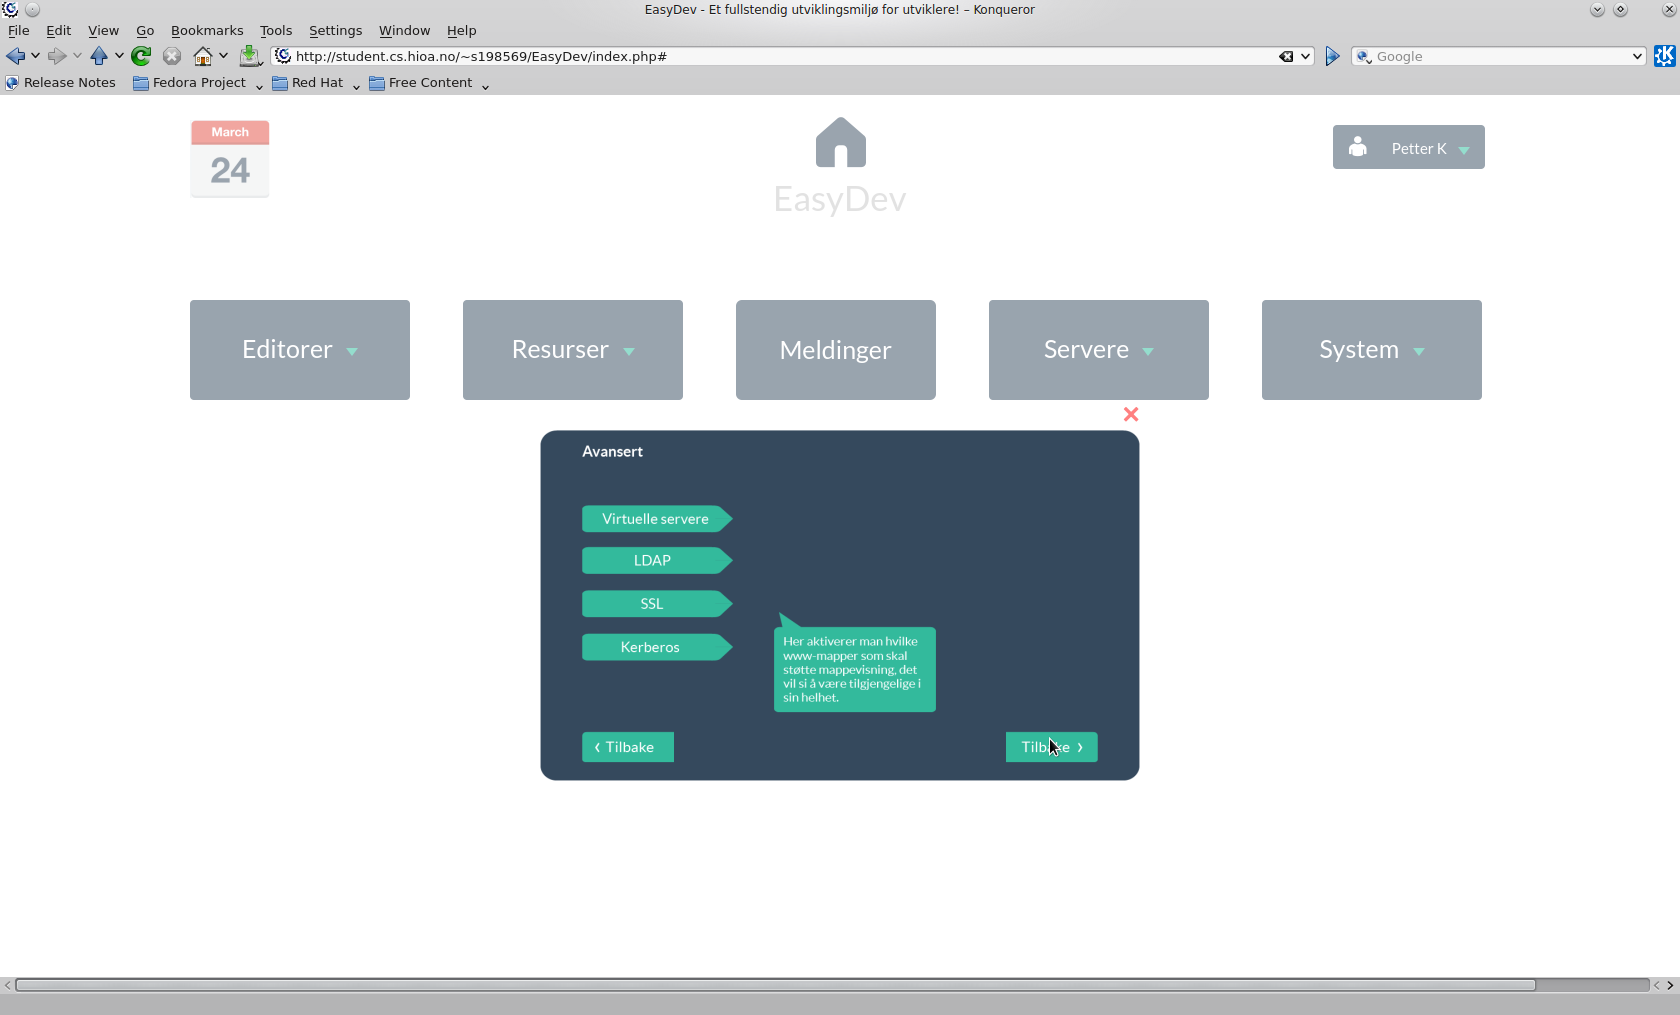
\includegraphics[width=\textwidth,height=\textheight,keepaspectratio]{./img/prosessdokumentasjon/hifi/a5.png}
\caption{(Hi-fi) Webserver:}
\label{fig:apachehi5}
\end{figure}

%KONFIGURASJON AV BRUKERE
\begin{figure}[ht]
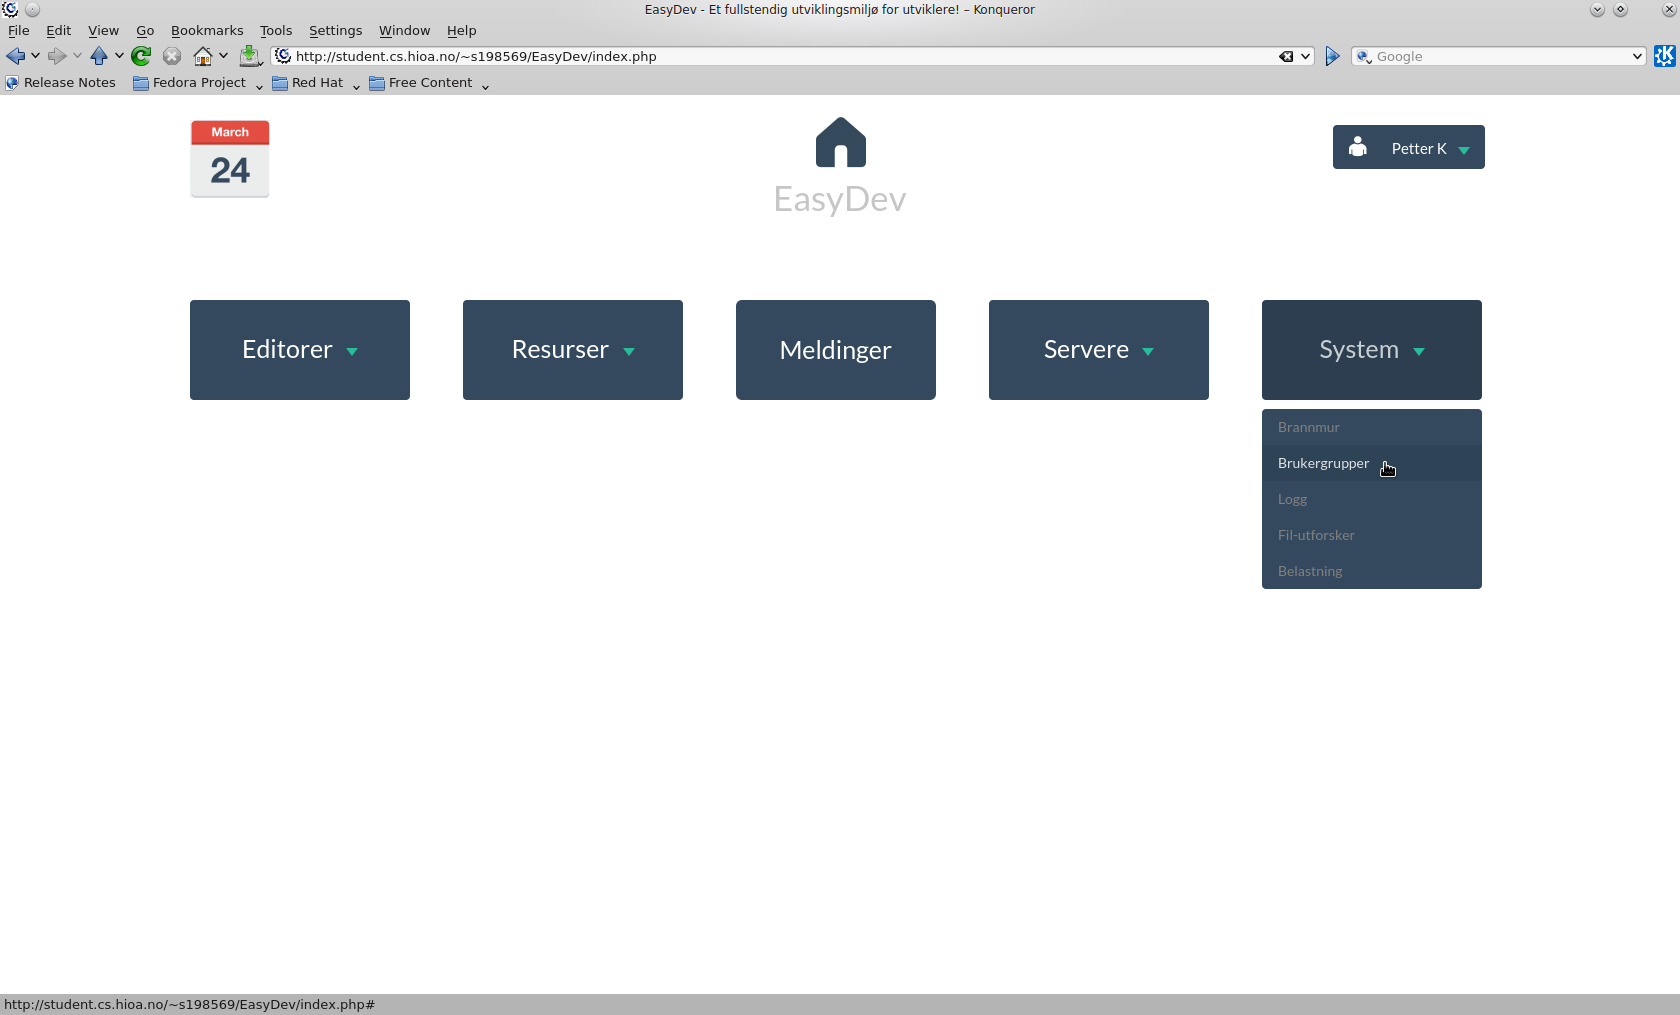
\includegraphics[width=\textwidth,height=\textheight,keepaspectratio]{./img/prosessdokumentasjon/hifi/b1.png}
\caption{Brukere: }
\label{fig:brukerehi1}
\end{figure}

\begin{figure}[ht]
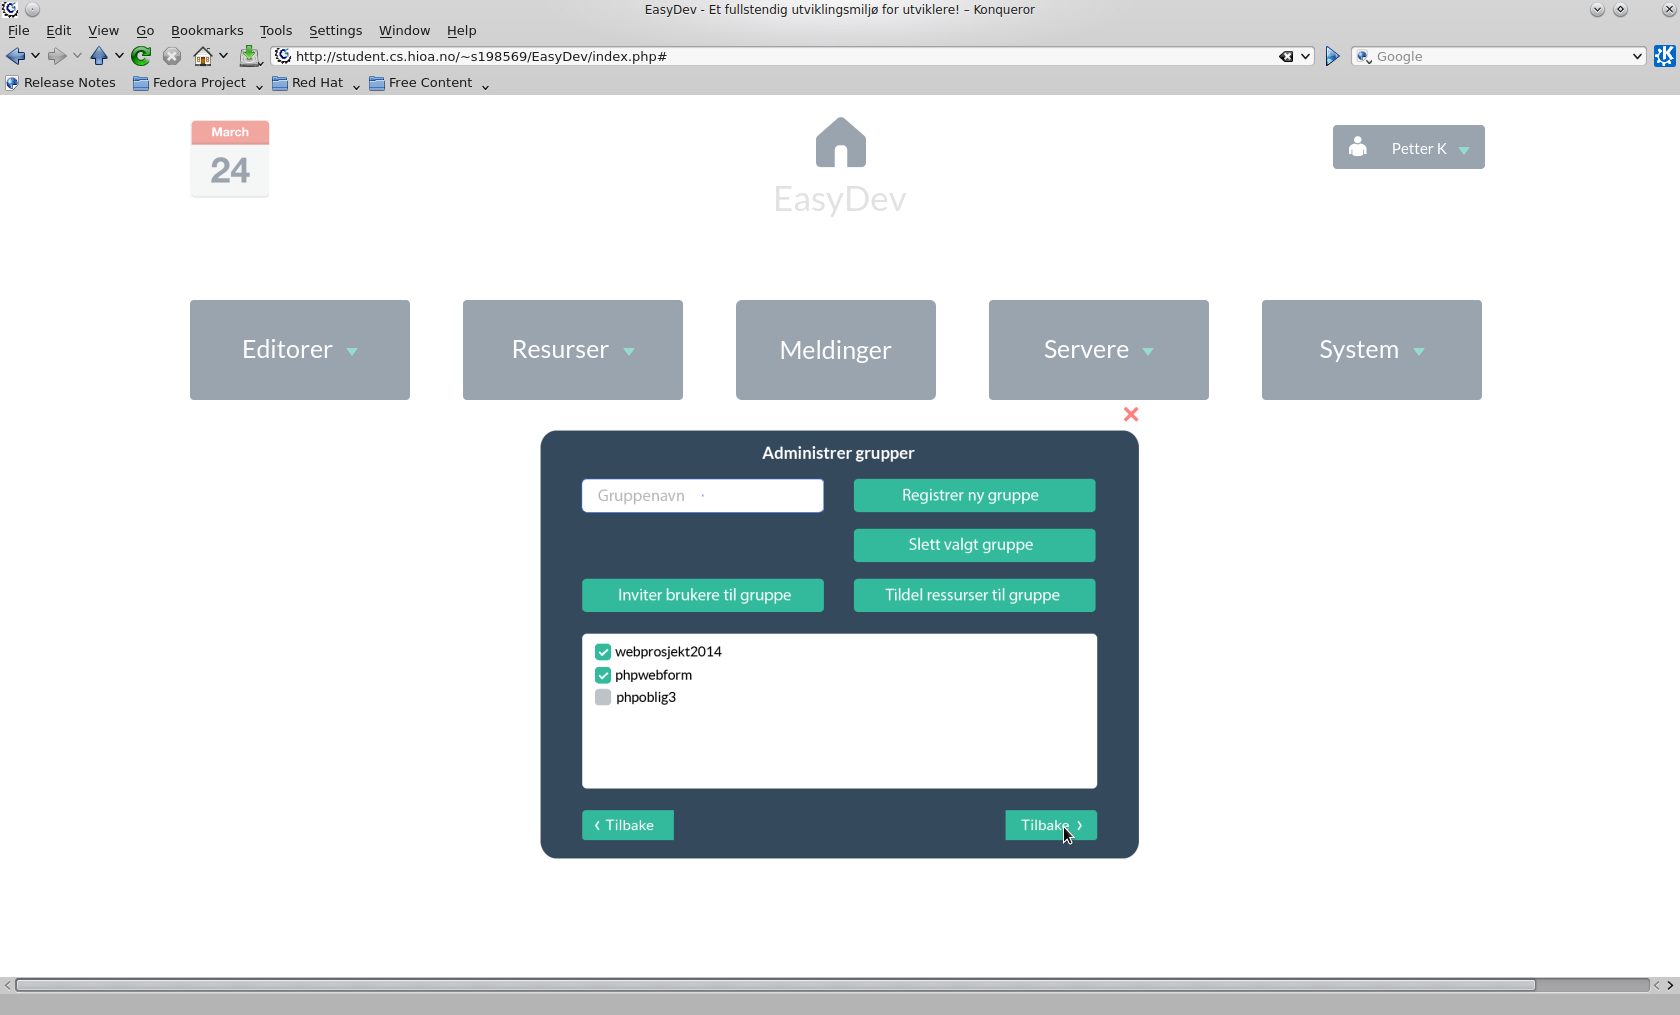
\includegraphics[width=\textwidth,height=\textheight,keepaspectratio]{./img/prosessdokumentasjon/hifi/b2.png}
\caption{Brukere: }
\label{fig:brukerehi2}
\end{figure}

\begin{figure}[ht]
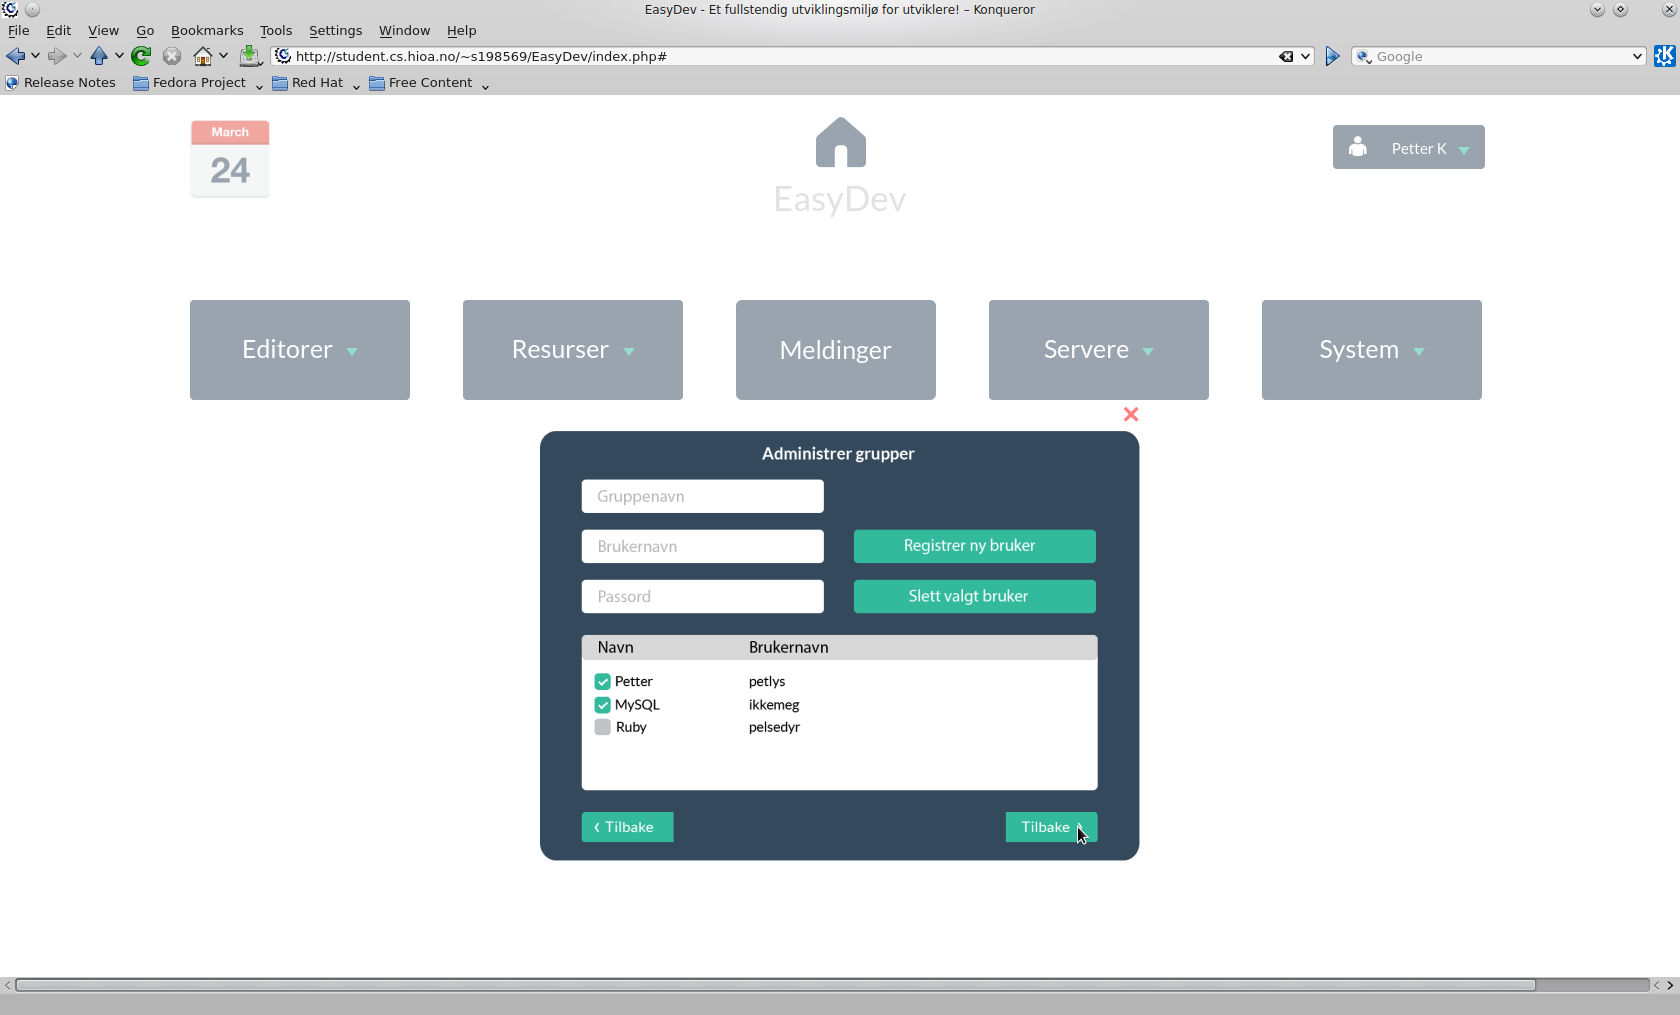
\includegraphics[width=\textwidth,height=\textheight,keepaspectratio]{./img/prosessdokumentasjon/hifi/b3.png}
\caption{Brukere: }
\label{fig:brukerehi3}
\end{figure}

\begin{figure}[ht]
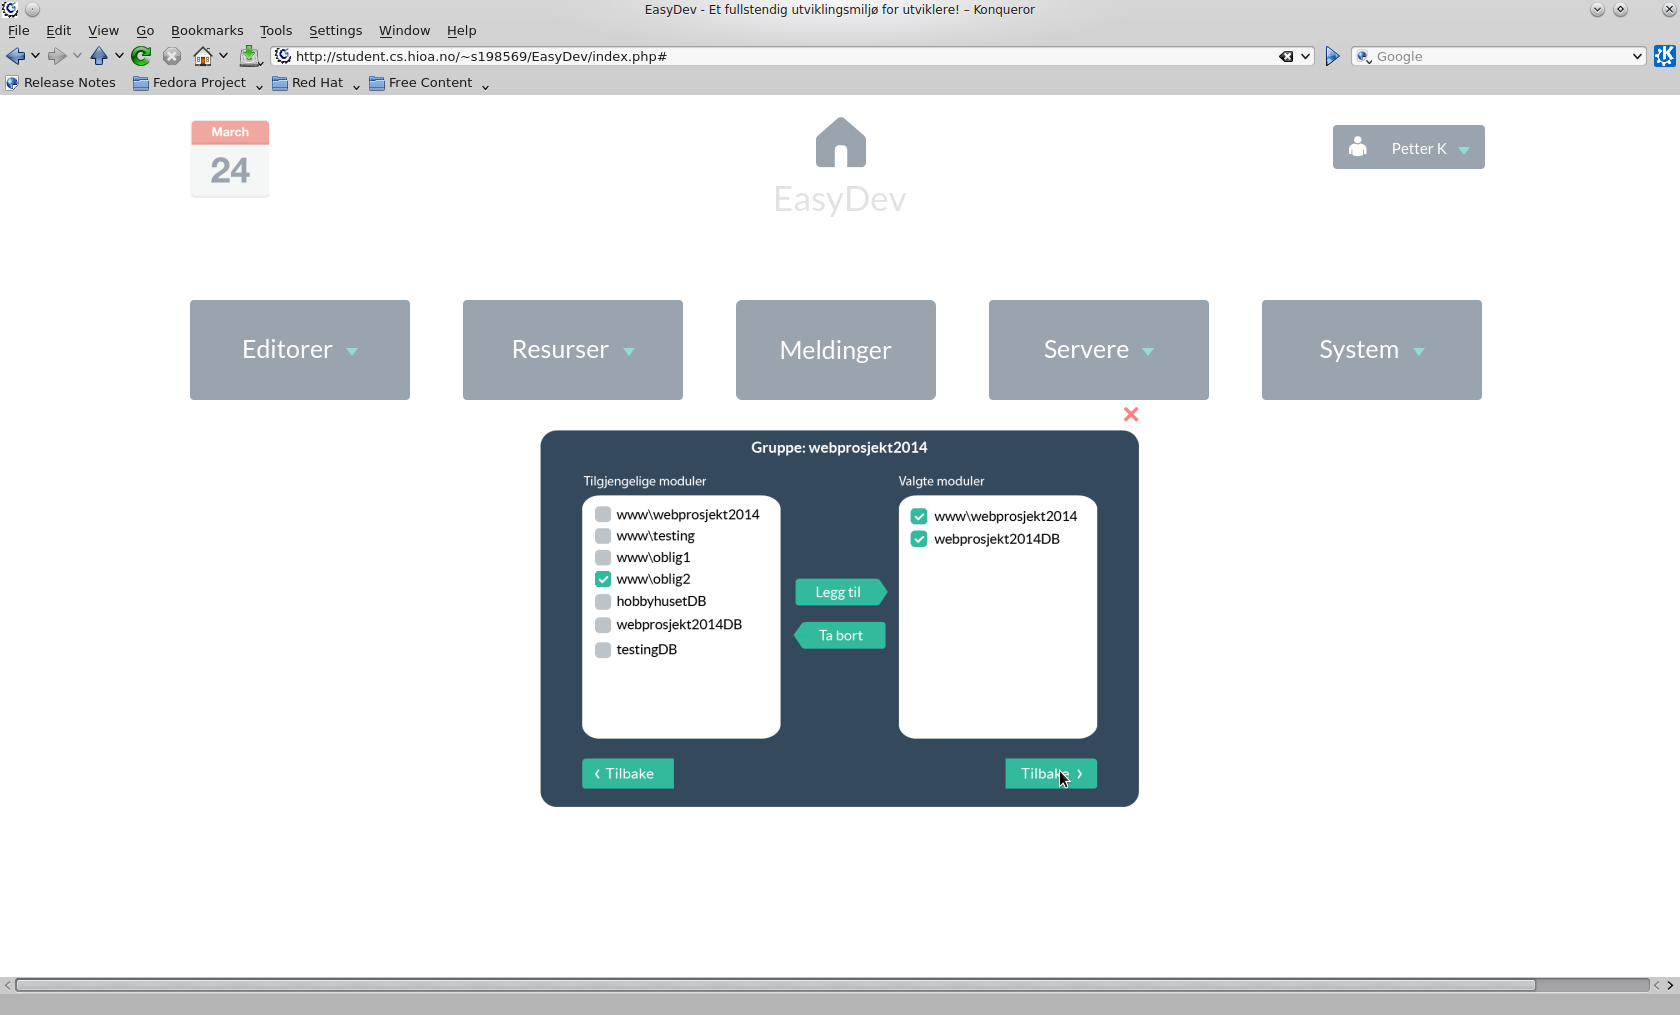
\includegraphics[width=\textwidth,height=\textheight,keepaspectratio]{./img/prosessdokumentasjon/hifi/b4.png}
\caption{Brukere: }
\label{fig:brukerehi4}
\end{figure}


% IKKE SLETT VIL HA DENNE SOM EKSEMPEL
%\begin{figure}[ht]
% 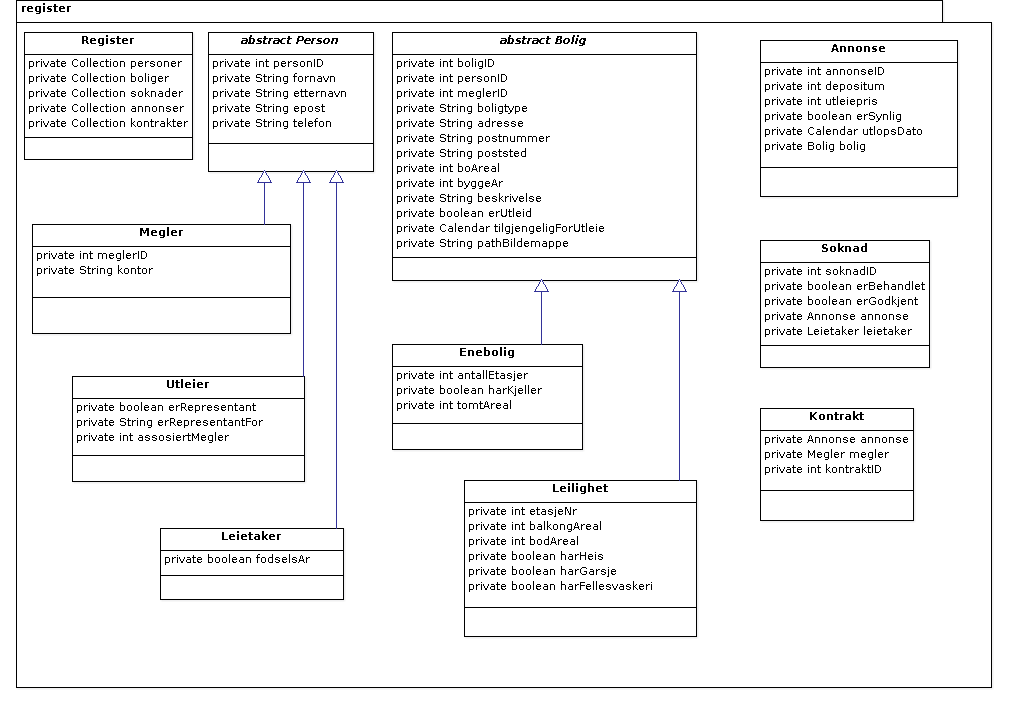
\includegraphics[angle=90 ,width=\textwidth,height=\textheight,keepaspectratio]{./img/appendix/diagram/klassestruktur_uml.png}
% \caption{Innledende UML diagram. brukt for generering av grunnleggende klasser.}
% %Her kommer en kabel for kryssreferering i teksten til figuren
% \label{fig:uml_diag}
%\end{figure}

\end{document}